% Needs to be done: electric layout
%                   ltspice simulation
%                   report
%% bare_conf.tex
%% V1.3
%% 2007/01/11
%% by Michael Shell
%% See:
%% http://www.michaelshell.org/
%% for current contact information.
%%
%% This is a skeleton file demonstrating the use of IEEEtran.cls
%% (requires IEEEtran.cls version 1.7 or later) with an IEEE conference paper.
%%
%% Support sites:
%% http://www.michaelshell.org/tex/ieeetran/
%% http://www.ctan.org/tex-archive/macros/latex/contrib/IEEEtran/
%% and
%% http://www.ieee.org/

%%*************************************************************************
%% Legal Notice:
%% This code is offered as-is without any warranty either expressed or
%% implied; without even the implied warranty of MERCHANTABILITY or
%% FITNESS FOR A PARTICULAR PURPOSE! 
%% User assumes all risk.
%% In no event shall IEEE or any contributor to this code be liable for
%% any damages or losses, including, but not limited to, incidental,
%% consequential, or any other damages, resulting from the use or misuse
%% of any information contained here.
%%
%% All comments are the opinions of their respective authors and are not
%% necessarily endorsed by the IEEE.
%%
%% This work is distributed under the LaTeX Project Public License (LPPL)
%% ( http://www.latex-project.org/ ) version 1.3, and may be freely used,
%% distributed and modified. A copy of the LPPL, version 1.3, is included
%% in the base LaTeX documentation of all distributions of LaTeX released
%% 2003/12/01 or later.
%% Retain all contribution notices and credits.
%% ** Modified files should be clearly indicated as such, including  **
%% ** renaming them and changing author support contact information. **
%%
%% File list of work: IEEEtran.cls, IEEEtran_HOWTO.pdf, bare_adv.tex,
%%                    bare_conf.tex, bare_jrnl.tex, bare_jrnl_compsoc.tex
%%*************************************************************************

% *** Authors should verify (and, if needed, correct) their LaTeX system  ***
% *** with the testflow diagnostic prior to trusting their LaTeX platform ***
% *** with production work. IEEE's font choices can trigger bugs that do  ***
% *** not appear when using other class files.                            ***
% The testflow support page is at:
% http://www.michaelshell.org/tex/testflow/

% Note that the a4paper option is mainly intended so that authors in
% countries using A4 can easily print to A4 and see how their papers will
% look in print - the typesetting of the document will not typically be
% affected with changes in paper size (but the bottom and side margins will).
% Use the testflow package mentioned above to verify correct handling of
% both paper sizes by the user's LaTeX system.
%
% Also note that the "draftcls" or "draftclsnofoot", not "draft", option
% should be used if it is desired that the figures are to be displayed in
% draft mode.
%
\documentclass[conference]{IEEEtran}
% Add the compsoc option for Computer Society conferences.
%
% If IEEEtran.cls has not been installed into the LaTeX system files,
% manually specify the path to it like:
% \documentclass[conference]{../sty/IEEEtran}





% Some very useful LaTeX packages include:
% (uncomment the ones you want to load)


% *** MISC UTILITY PACKAGES ***
%
%\usepackage{ifpdf}
% Heiko Oberdiek's ifpdf.sty is very useful if you need conditional
% compilation based on whether the output is pdf or dvi.
% usage:
% \ifpdf
%   % pdf code
% \else
%   % dvi code
% \fi
% The latest version of ifpdf.sty can be obtained from:
% http://www.ctan.org/tex-archive/macros/latex/contrib/oberdiek/
% Also, note that IEEEtran.cls V1.7 and later provides a builtin
% \ifCLASSINFOpdf conditional that works the same way.
% When switching from latex to pdflatex and vice-versa, the compiler may
% have to be run twice to clear warning/error messages.




% *** CITATION PACKAGES ***
%
\usepackage{cite}
% cite.sty was written by Donald Arseneau
% V1.6 and later of IEEEtran pre-defines the format of the cite.sty package
% \cite{} output to follow that of IEEE. Loading the cite package will
% result in citation numbers being automatically sorted and properly
% "compressed/ranged". e.g., [1], [9], [2], [7], [5], [6] without using
% cite.sty will become [1], [2], [5]--[7], [9] using cite.sty. cite.sty's
% \cite will automatically add leading space, if needed. Use cite.sty's
% noadjust option (cite.sty V3.8 and later) if you want to turn this off.
% cite.sty is already installed on most LaTeX systems. Be sure and use
% version 4.0 (2003-05-27) and later if using hyperref.sty. cite.sty does
% not currently provide for hyperlinked citations.
% The latest version can be obtained at:
% http://www.ctan.org/tex-archive/macros/latex/contrib/cite/
% The documentation is contained in the cite.sty file itself.






% *** GRAPHICS RELATED PACKAGES ***
%
\ifCLASSINFOpdf
   \usepackage[pdftex]{graphicx}
  % declare the path(s) where your graphic files are
  % \graphicspath{{../pdf/}{../jpeg/}}
  % and their extensions so you won't have to specify these with
  % every instance of \includegraphics
  % \DeclareGraphicsExtensions{.pdf,.jpeg,.png}
\else
  % or other class option (dvipsone, dvipdf, if not using dvips). graphicx
  % will default to the driver specified in the system graphics.cfg if no
  % driver is specified.
   \usepackage[dvips]{graphicx}
  % declare the path(s) where your graphic files are
  % \graphicspath{{../eps/}}
  % and their extensions so you won't have to specify these with
  % every instance of \includegraphics
  % \DeclareGraphicsExtensions{.eps}
\fi
% graphicx was written by David Carlisle and Sebastian Rahtz. It is
% required if you want graphics, photos, etc. graphicx.sty is already
% installed on most LaTeX systems. The latest version and documentation can
% be obtained at: 
% http://www.ctan.org/tex-archive/macros/latex/required/graphics/
% Another good source of documentation is "Using Imported Graphics in
% LaTeX2e" by Keith Reckdahl which can be found as epslatex.ps or
% epslatex.pdf at: http://www.ctan.org/tex-archive/info/
%
% latex, and pdflatex in dvi mode, support graphics in encapsulated
% postscript (.eps) format. pdflatex in pdf mode supports graphics
% in .pdf, .jpeg, .png and .mps (metapost) formats. Users should ensure
% that all non-photo figures use a vector format (.eps, .pdf, .mps) and
% not a bitmapped formats (.jpeg, .png). IEEE frowns on bitmapped formats
% which can result in "jaggedy"/blurry rendering of lines and letters as
% well as large increases in file sizes.
%
% You can find documentation about the pdfTeX application at:
% http://www.tug.org/applications/pdftex


\usepackage{float}
%\restylefloat{table}
\usepackage{pbox}
\usepackage{hyperref}
% *** MATH PACKAGES ***
%
\usepackage[cmex10]{amsmath}
\usepackage{amssymb}
\usepackage{exscale,relsize}
% A popular package from the American Mathematical Society that provides
% many useful and powerful commands for dealing with mathematics. If using
% it, be sure to load this package with the cmex10 option to ensure that
% only type 1 fonts will utilized at all point sizes. Without this option,
% it is possible that some math symbols, particularly those within
% footnotes, will be rendered in bitmap form which will result in a
% document that can not be IEEE Xplore compliant!
%
% Also, note that the amsmath package sets \interdisplaylinepenalty to 10000
% thus preventing page breaks from occurring within multiline equations. Use:
%\interdisplaylinepenalty=2500
% after loading amsmath to restore such page breaks as IEEEtran.cls normally
% does. amsmath.sty is already installed on most LaTeX systems. The latest
% version and documentation can be obtained at:
% http://www.ctan.org/tex-archive/macros/latex/required/amslatex/math/





% *** SPECIALIZED LIST PACKAGES ***
%
%\usepackage{algorithmic}
% algorithmic.sty was written by Peter Williams and Rogerio Brito.
% This package provides an algorithmic environment fo describing algorithms.
% You can use the algorithmic environment in-text or within a figure
% environment to provide for a floating algorithm. Do NOT use the algorithm
% floating environment provided by algorithm.sty (by the same authors) or
% algorithm2e.sty (by Christophe Fiorio) as IEEE does not use dedicated
% algorithm float types and packages that provide these will not provide
% correct IEEE style captions. The latest version and documentation of
% algorithmic.sty can be obtained at:
% http://www.ctan.org/tex-archive/macros/latex/contrib/algorithms/
% There is also a support site at:
% http://algorithms.berlios.de/index.html
% Also of interest may be the (relatively newer and more customizable)
% algorithmicx.sty package by Szasz Janos:
% http://www.ctan.org/tex-archive/macros/latex/contrib/algorithmicx/




% *** ALIGNMENT PACKAGES ***
%
\usepackage{array}
% Frank Mittelbach's and David Carlisle's array.sty patches and improves
% the standard LaTeX2e array and tabular environments to provide better
% appearance and additional user controls. As the default LaTeX2e table
% generation code is lacking to the point of almost being broken with
% respect to the quality of the end results, all users are strongly
% advised to use an enhanced (at the very least that provided by array.sty)
% set of table tools. array.sty is already installed on most systems. The
% latest version and documentation can be obtained at:
% http://www.ctan.org/tex-archive/macros/latex/required/tools/


%\usepackage{mdwmath}
%\usepackage{mdwtab}
% Also highly recommended is Mark Wooding's extremely powerful MDW tools,
% especially mdwmath.sty and mdwtab.sty which are used to format equations
% and tables, respectively. The MDWtools set is already installed on most
% LaTeX systems. The lastest version and documentation is available at:
% http://www.ctan.org/tex-archive/macros/latex/contrib/mdwtools/


% IEEEtran contains the IEEEeqnarray family of commands that can be used to
% generate multiline equations as well as matrices, tables, etc., of high
% quality.


%\usepackage{eqparbox}
% Also of notable interest is Scott Pakin's eqparbox package for creating
% (automatically sized) equal width boxes - aka "natural width parboxes".
% Available at:
% http://www.ctan.org/tex-archive/macros/latex/contrib/eqparbox/





% *** SUBFIGURE PACKAGES ***
\usepackage[tight,footnotesize]{subfigure}
% subfigure.sty was written by Steven Douglas Cochran. This package makes it
% easy to put subfigures in your figures. e.g., "Figure 1a and 1b". For IEEE
% work, it is a good idea to load it with the tight package option to reduce
% the amount of white space around the subfigures. subfigure.sty is already
% installed on most LaTeX systems. The latest version and documentation can
% be obtained at:
% http://www.ctan.org/tex-archive/obsolete/macros/latex/contrib/subfigure/
% subfigure.sty has been superceeded by subfig.sty.



%\usepackage[caption=false]{caption}
%\usepackage[font=footnotesize]{subfig}
% subfig.sty, also written by Steven Douglas Cochran, is the modern
% replacement for subfigure.sty. However, subfig.sty requires and
% automatically loads Axel Sommerfeldt's caption.sty which will override
% IEEEtran.cls handling of captions and this will result in nonIEEE style
% figure/table captions. To prevent this problem, be sure and preload
% caption.sty with its "caption=false" package option. This is will preserve
% IEEEtran.cls handing of captions. Version 1.3 (2005/06/28) and later 
% (recommended due to many improvements over 1.2) of subfig.sty supports
% the caption=false option directly:
%\usepackage[caption=false,font=footnotesize]{subfig}
%
% The latest version and documentation can be obtained at:
% http://www.ctan.org/tex-archive/macros/latex/contrib/subfig/
% The latest version and documentation of caption.sty can be obtained at:
% http://www.ctan.org/tex-archive/macros/latex/contrib/caption/




% *** FLOAT PACKAGES ***
%
\usepackage{fixltx2e}
% fixltx2e, the successor to the earlier fix2col.sty, was written by
% Frank Mittelbach and David Carlisle. This package corrects a few problems
% in the LaTeX2e kernel, the most notable of which is that in current
% LaTeX2e releases, the ordering of single and double column floats is not
% guaranteed to be preserved. Thus, an unpatched LaTeX2e can allow a
% single column figure to be placed prior to an earlier double column
% figure. The latest version and documentation can be found at:
% http://www.ctan.org/tex-archive/macros/latex/base/



%\usepackage{stfloats}
% stfloats.sty was written by Sigitas Tolusis. This package gives LaTeX2e
% the ability to do double column floats at the bottom of the page as well
% as the top. (e.g., "\begin{figure*}[!b]" is not normally possible in
% LaTeX2e). It also provides a command:
%\fnbelowfloat
% to enable the placement of footnotes below bottom floats (the standard
% LaTeX2e kernel puts them above bottom floats). This is an invasive package
% which rewrites many portions of the LaTeX2e float routines. It may not work
% with other packages that modify the LaTeX2e float routines. The latest
% version and documentation can be obtained at:
% http://www.ctan.org/tex-archive/macros/latex/contrib/sttools/
% Documentation is contained in the stfloats.sty comments as well as in the
% presfull.pdf file. Do not use the stfloats baselinefloat ability as IEEE
% does not allow \baselineskip to stretch. Authors submitting work to the
% IEEE should note that IEEE rarely uses double column equations and
% that authors should try to avoid such use. Do not be tempted to use the
% cuted.sty or midfloat.sty packages (also by Sigitas Tolusis) as IEEE does
% not format its papers in such ways.





% *** PDF, URL AND HYPERLINK PACKAGES ***
%
%\usepackage{url}
% url.sty was written by Donald Arseneau. It provides better support for
% handling and breaking URLs. url.sty is already installed on most LaTeX
% systems. The latest version can be obtained at:
% http://www.ctan.org/tex-archive/macros/latex/contrib/misc/
% Read the url.sty source comments for usage information. Basically,
% \url{my_url_here}.


\newcommand{\tab}{\hspace*{2em}}
%tab command definition

\usepackage{booktabs}
%thicker hlines

% *** Do not adjust lengths that control margins, column widths, etc. ***
% *** Do not use packages that alter fonts (such as pslatex).         ***
% There should be no need to do such things with IEEEtran.cls V1.6 and later.
% (Unless specifically asked to do so by the journal or conference you plan
% to submit to, of course. )


% correct bad hyphenation here
\hyphenation{op-tical net-works semi-conduc-tor}

%\DeclareMathSizes{ds}{ts}{ss}{sss}, where ds is the display size, ts is the text size, etc.
%\DeclareMathSizes{10}{18}{12}{8} 
%\everymath{\displaystyle}
\begin{document}
%
% paper title
% can use linebreaks \\ within to get better formatting as desired
\title{Bandgap Voltage Reference Project}

\author{\IEEEauthorblockN{Marc Christiansen}
\IEEEauthorblockA{Email: mjch@pdx.edu}\\
\and
\IEEEauthorblockN{Jackson Pugh}
\IEEEauthorblockA{%IEEE Student Member and Officer\\
Email: japugh@pdx.edu}
\and
\IEEEauthorblockN{Krish Ramkumar}
\IEEEauthorblockA{Email: krish13007@gmail.com}}

\maketitle

\begin{abstract}
Write this after the paper has been finished.
\end{abstract}
\IEEEpeerreviewmaketitle

\section{Introduction}
\IEEEPARstart{V}{oltage} references play a critical role in analog and digital circuits.  Fig. \ref{fig:overview} illustrates the relationships between each module found in analog circuits.
\begin{figure}[!htbp]
  \centering
  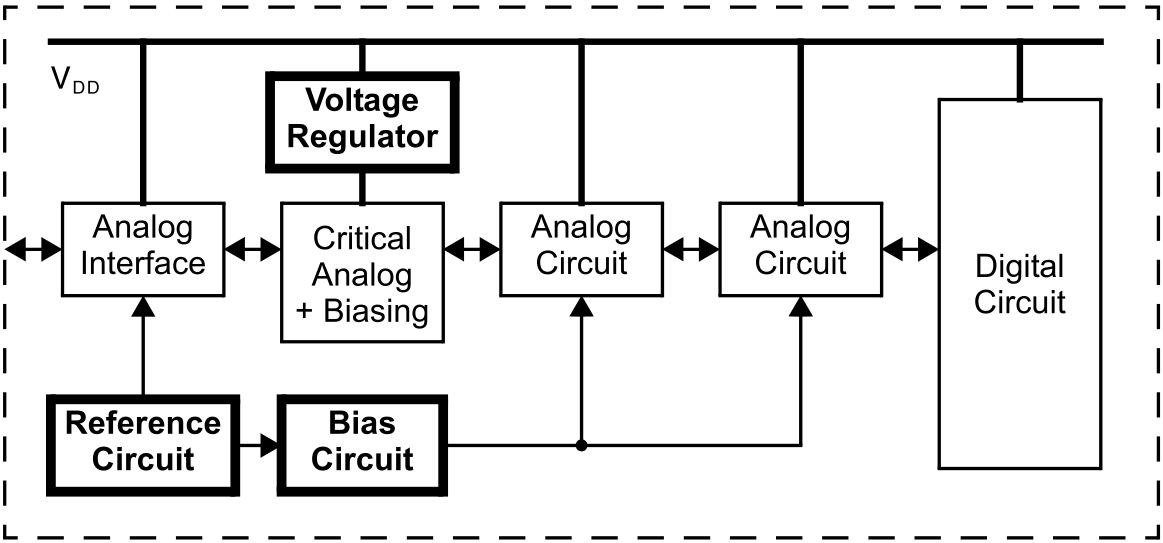
\includegraphics[scale=0.25]{images/overview.png}
  \caption[Overview]{Overview of modules found in analog circuits.\footnotemark}
  \label{fig:overview}
\end{figure}
\footnotetext{Image taken from Analog Integrated Circuit Design 2nd Ed. by Carusone}
\\Ideally, voltage references provide constant voltage regardless of changes in temperature, supply voltage, or load.  This is important for subsystems which depend on a fixed voltage where the environmental conditions are not constant.  Examples include ADC/DAC, voltage regulators, measurement, and control systems.
\subsection{Design Tools, Set Up and Assumptions}
The following tools, settings, and assumptions were used.
\begin{itemize}
  \item LTspice IV
  \item Electric VLSI Design System
  \item MATLAB
  \item 0.18$\mu$m CMOS technology based off the Analog Integrated Circuit Design 2nd Ed. course website\footnote{\href{http://analogicdesign.com/students/netlists-models/model-files/}{Analog Integrated Circuit Design 2nd Ed. Model Files}} website
  \item Temperature range between -50 to 100 $^\circ$C
  \item Ideal voltage/current source
  \item Ideal operational amplifier
\end{itemize}

\subsection{Design Objectives}
The main objectives for the voltage reference design are
\begin{enumerate}
  \item Minimize $TC(V_{_{ref}})$\;(temperature coefficient)
  \item Minimize $V_{DD}$ sensitivity
  \item Minimize $P$ consumption
\end{enumerate}
These design objectives are achieved using an iterative approach.  The layout is done only for the MOSFET-Only Voltage Divider.

\subsection{Design Methodology}
Our design methodology is outlined in the flowchart show in Figure \ref{fig:design-methodology}.  For each circuit topology, we will: develop the necessary design equations/assumptions, size the circuit components, simulate the circuits in LTSpice, and evaluate the simulation results.  If the results do not meet our design objectives, then we will examine our design equations/assumptions, resize the circuit components, and re-run the simulations.  If the results meet our design objectives, then we move onto the next circuit.
\begin{figure}[!htbp]
  \centering
  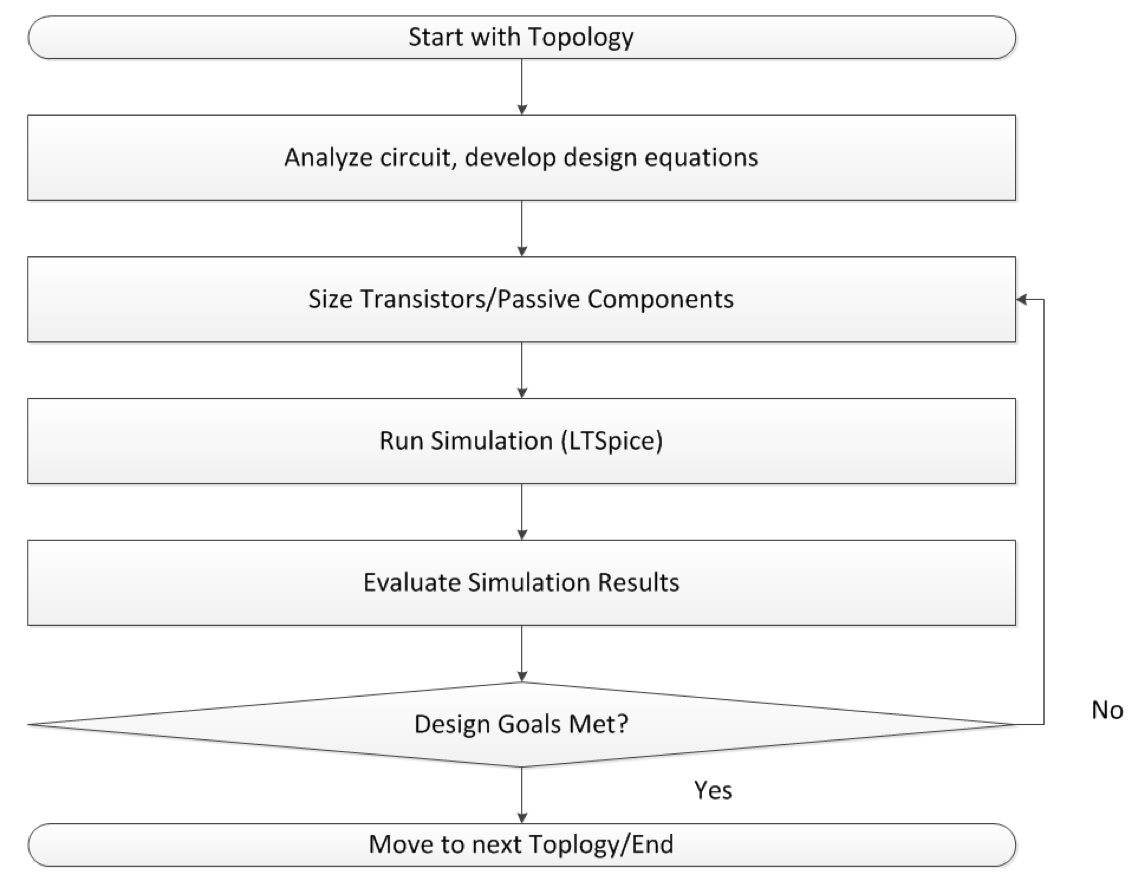
\includegraphics[scale=0.45]{images/design-methodology.png}
  \caption[design-methodology]{Design Methodology}
  \label{fig:design-methodology}
\end{figure}
\\\tab
For the MOSFET-Only circuit topology, we will also layout and simulate the design in Electric.  If the simulation results meet our design requirements, we will move on to the next topology.  Otherwise, we will iterate the design as is done for the rest of the circuit topologies.\\

\subsection{Design Topologies}
Four different voltage reference topologies are investigated.
\subsubsection{Design 1. Resistor-MOSFET Voltage Divider}
The most basic design.  This design should be good for first-order effects but simulation performance may suffer when higher-order parameters are included.
\subsubsection{Design 2. MOSFET-Only Voltage Divider}
Improved design.  This design should have a better temperature coefficient than the Resistor-MOSFET design since the P-channel MOSFET load adds an additonal degree of freedom.
\subsubsection{Design 3. Current-Diode Voltage Reference}
Improved design.  This topology should perform well in simulation, however this circuit is difficult to realize due to the reliance on an absolute, ideal current source which is nearly impossible to design and impliment.\\
\tab\emph{Note: Designs 1-3 will be designed and tested without consideration of next-stage loading effects.  Section \ref{sec:Buff} discusses how to minimize these effects on the reference voltage.}
\subsubsection{Design 4. CMOS Bandgap Voltage Reference}
Advanced design; based on the Brokaw Bandgap Reference.  This design is implemented using vertical CMOS diode-connected PNP BJTs and an ideal operational amplifier; it will be verified that the ideal op amp is performing within a reasonable approximation of a real op amp.
\subsection{Global Design Parameters}
The following parameters are used in the calculations for each circuit topology.
\begin{itemize}
  \item $V_{_{DD}} = 1.8\;\mathrm{V}$ \emph{(except in Design 4 where $V_{_{DD}} = 3.3\;\mathrm{V}$)}
  \item $TC_{_R} = 2,000\;\mathrm{ppm}\;(0.002)$
	\item $T_0 = 20\;^{\circ} C$
\end{itemize}
\begin{table}[!htbp]
  \caption[]{Parameters for calculations}
  \label{tab:parameters}
  \centering
  \begin{tabular}{|l|l|l|l|}
    \hline
    Parameter                       & NMOS    & PMOS	&PNP Diode     \\ \hline
    $V_{_{to}}$ (V)                   & 0.45    & -0.45	&-      \\ 
    $K_{_n}$ ($\mu$A/V$^2$)               & 270     & 70 	&-        \\ 
    ${\lambda}{\cdot}L$ ($\mu$m/V)  & 0.08    & 0.08	&-       \\
    $I_S$ ($A$)				&-	&-	&1e$-18$\\
    $TC(V_{TP,TN})$		&3,000 $ppm$ &3,000 $ppm$	&-	\\
    %        ~          & ~    & ~    \\
    \hline
  \end{tabular}
\end{table}
\newpage
%%Resistor-MOS Begin
\section{Resistor-MOSFET Voltage Divider}
Design 1 consists of a diode connected N-channel MOSFET with a resistive load.  The resistive load has a positive temperature coefficient while the N-channel MOSFET has a negative temperature coefficient.  This relationship allows for close-to-constant output voltage based on proper sizing of the devices.\\\tab
Figure \ref{fig:resistor-mosfet1} shows the basic circuit topology.  This is a simple resistor-MOSEFT voltage divider without consideration for loading effects.  Figure \ref{fig:resistor-mosfet1-ss} shows the small signal circuit equivalent for the resistor-MOSFET divider.
\begin{figure}[!htbp]
  \centering
  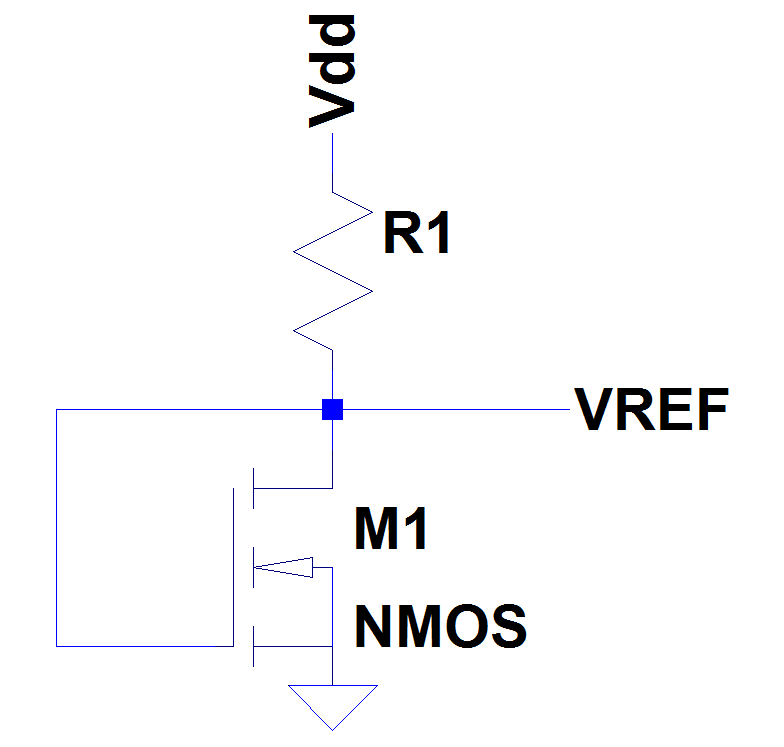
\includegraphics[scale=0.25]{images/resistor-mosfet1.png}
  \caption[resistor1]{Resistor-MOSFET Circuit}
  \label{fig:resistor-mosfet1}
\end{figure}
\begin{figure}[!htbp]
  \centering
  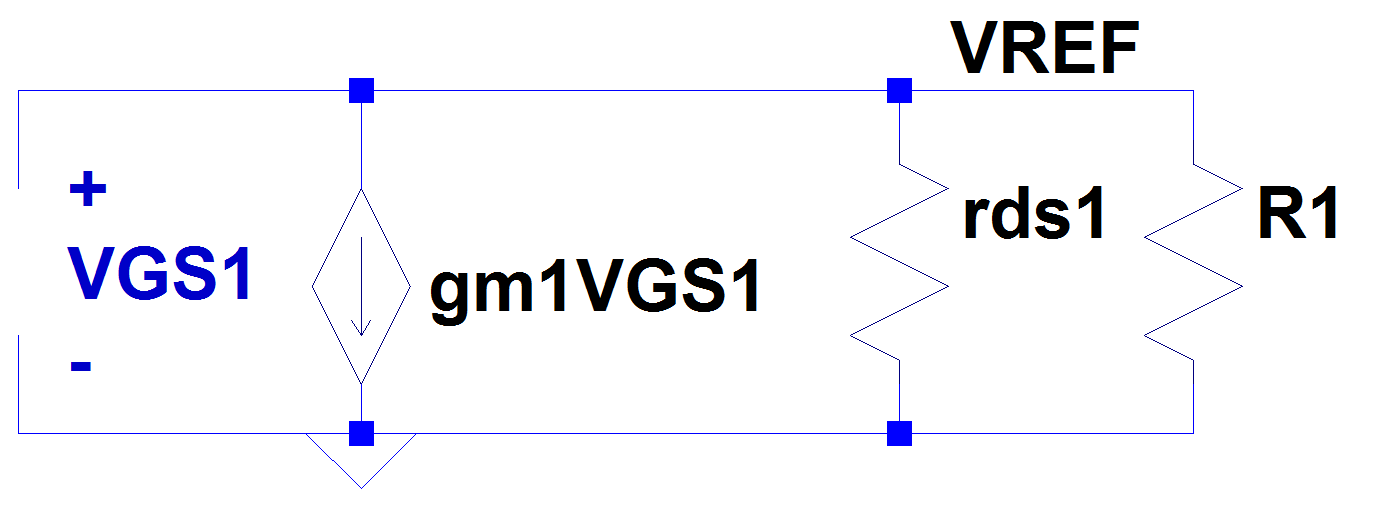
\includegraphics[scale=0.25]{images/resistor-mosfet1-ss.png}
  \caption[resistor1-ss]{Resistor-MOSFET Small Signal Circuit}
  \label{fig:resistor-mosfet1-ss}
\end{figure}

\subsection{Resistor-MOSFET Design Equations} 
Table \ref{tab:resistor-mosfet-designequations} gives the design equations used throughout the design of the Resistor-MOSFET Voltage Divider.
\begin{table}[!htbp]
  \caption[]{Resistor-MOSFET Design Equations}
  \label{tab:resistor-mosfet-designequations}
  \centering
  \begin{tabular}{|m{1.5cm}|m{6.5cm}|}
    \hline
    \pbox{1.5cm}{{\small Voltage Reference}} &
    \begin{equation}
      \label{r_ref}
      \mathsmaller{V_{_{REF}} = V_{_{TN}} - \sqrt{\frac{2(V_{_{DD}}-V_{_{REF}})}{RK_{_n}}}}
    \end{equation}\\
    \hline
	\pbox{1.5cm}{{\smaller Transconductance Parameter}} &
    \begin{equation}
      \label{rm-kpt}
      \mathsmaller{KP(T)=KP(T_{_0})(\frac{T}{T_0})^{-1.5}}
    \end{equation}\\
    \hline
    \pbox{1.5cm}{{\small $V_{_{DD}}$ Sensitivity}} &
      \begin{IEEEeqnarray}{rCl}
        \label{r_sensitivity}
        \mathsmaller{S_{_{VDD}}^{^{V{REF}}}} & \mathsmaller{=} & \mathsmaller{\frac{V_{_{DD}}}{V_{_{REF}}}\frac{\partial{V_{_{REF}}}}{\partial{V_{_{DD}}}}}
        \nonumber\\
        & \mathsmaller{\approx} & \mathsmaller{\frac{1}{V_{_{TN}}\sqrt{\frac{2RK_{_n}}{V_{_{DD}}}}+2}}
        \IEEEyesnumber
      \end{IEEEeqnarray}\\
    \hline
    \pbox{1.5cm}{{\small Temperature Coefficient}} &
    \begin{multline}
      \label{r_tc}
      \mathsmaller{TC_{_{REF}} = \frac{1}{V_{_{REF}}}\frac{\partial{V_{_{REF}}}}{\partial{T}}}\\\mathsmaller{=\frac{1}{V_{_{REF}}}\bigg[V_{_{TN}}TC_{_{V_{TN}}}-}\\\mathsmaller{\frac{1}{2}\sqrt{\frac{2L}{W}\frac{V_{_{DD}}}{RKP(T)}}{\cdot}\left[\frac{1}{R}{\cdot}\frac{{\partial}R}{{\partial}T}-\frac{1.5}{T}\right]\bigg]}
    \end{multline}\\
    \hline
	\pbox{1.5cm}{{\small Power Consumption}} &
    \begin{equation}
      \label{rm-P}
      \mathsmaller{P = IV}
    \end{equation}\\
    \hline
  \end{tabular}
\end{table}

\subsection{Iteration 1}
\subsubsection{Device Sizes}
Table \ref{tab:rm-ds-1} gives the device sizes for iteration 1 of the Resistor-MOSFET circuit topology.
\begin{table}[!htbp]
  \caption[]{Resistor-MOSFET Device Sizes, Iteration 1}
  \label{tab:rm-ds-1}
  \centering
  \begin{tabular}{|l|l|l|}
    \hline
    Parameter			& NMOS	&R1 \\ \hline
    $W$ ($\mu$m)		&3		&-\\ 
    $L$ ($\mu$m)		& 1		&-\\
    $R$ ($\Omega$)		&-		&2k\\
    %        ~          & ~    & ~    \\
    \hline
  \end{tabular}
\end{table}

\subsection{Iteration 2}
\subsubsection{Device Sizes}
Table \ref{tab:rm-ds-2} gives the device sizes for iteration 2 of the Resistor-MOSFET circuit topology. 
\begin{table}[!htbp]
  \caption[]{Resistor-MOSFET Device Sizes, Iteration 2}
  \label{tab:rm-ds-2}
  \centering
  \begin{tabular}{|l|l|l|}
    \hline
    Parameter			& NMOS	&R1 \\ \hline
    $W$ ($\mu$m)		&3		&-\\ 
    $L$ ($\mu$m)		& 1		&-\\
    $R$ ($\Omega$)		&-		&823k\\
    %        ~          & ~    & ~    \\
    \hline
  \end{tabular}
\end{table}
%%Resistor-MOS END
\pagebreak
%%MOS-ONLY Begin
\section{MOSFET-Only Voltage Divider}
The MOSFET-Only Voltage Divider topology is shown in Figure \ref{fig:mosfet-only1}.  This topology similar to the Resistor-MOSFET topolgy, but R1 is replaced with a diode connected PMOS transistor as an active load.  Figure \ref{fig:mosfet-only1-ss} shows the small signal circuit equivalent for the MOSFET-Only Voltage Divider.

\begin{figure}[!htbp]
  \centering
  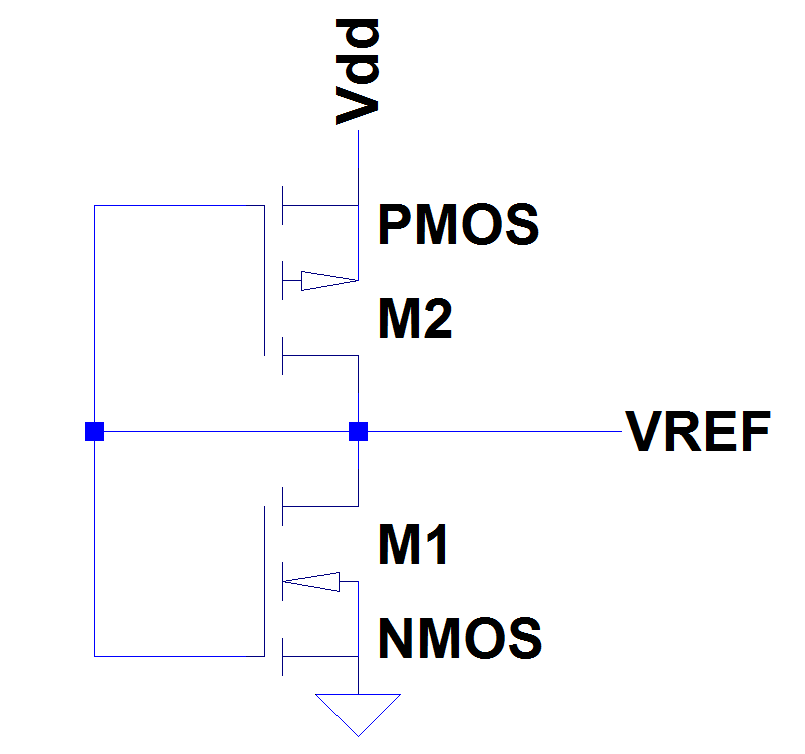
\includegraphics[scale=0.25]{images/mosfet-only1.png}
  \caption[mosfet-only1]{MOSFET-Only Circuit}
  \label{fig:mosfet-only1}
\end{figure}

\begin{figure}[!htbp]
  \centering
  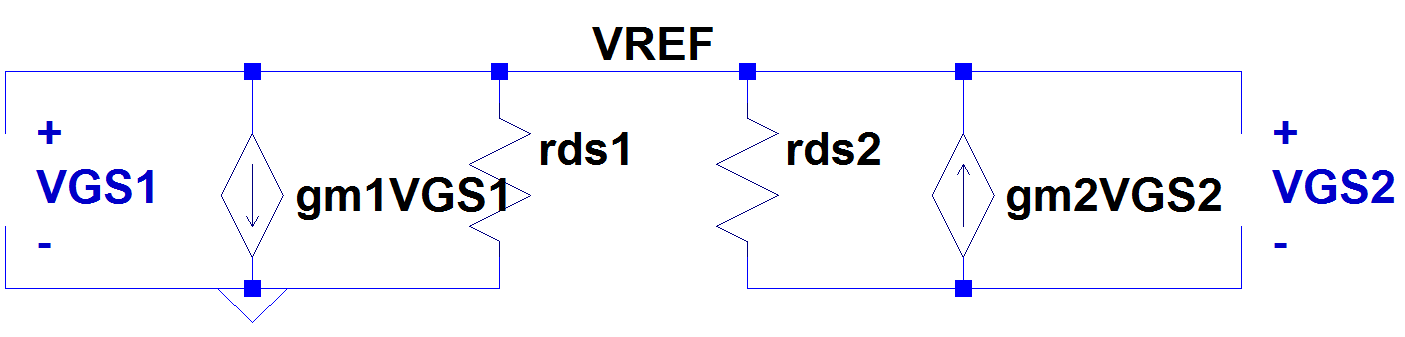
\includegraphics[scale=0.25]{images/mosfet-only1-ss.png}
  \caption[mosfet-only1-ss]{MOSFET-Only Small Signal Circuit}
  \label{fig:mosfet-only1-ss}
\end{figure}
\subsection{MOSFET-Only Design Approach}
Table \ref{tab:mosfet-only-designequations} gives the design equations used throughout the design of the MOSFET-Only Voltage Divider.  The design approach for the MOSFET-Only voltage divider is as follows:
\begin{enumerate}
  \item Develop the equations for the $V_{ref}$ and $TC(V_{ref})$.
  \item Set the addition argument in (\ref{mo-tc1}) $=0$.
  \item Solve for the ratio $\sqrt{\frac{K_n}{K_p}}$.
\end{enumerate}

Equation \ref{mo-tc1} is developed under the assumption that $\frac{\partial{V_{TP,TN}}}{\partial{T}} >> \frac{\partial{K_{n,p}}}{\partial{T}}$.  Since $TC(V_{TP})=TC(V_{TN})$ and $|{V_{TN}}|=|V_{TP}|$, the ratio $\frac{K_n}{K_p} = 1$.  This also implies that $gm_1=gm_2$; thus, the output impedance is given by (\ref{mo-ro}).

\begin{table}[!htbp]
  \caption[]{MOSFET-Only Design Equations}
  \label{tab:mosfet-only-designequations}
  \centering
  \begin{tabular}{|m{1.5cm}|m{6.5cm}|}
    \hline
\pbox{1.5cm}{{\small Design Contstraints}}
    &
    \begin{equation}
      \mathsmaller{V_{_{GS1}} = V_{_{GS2}} = V_{_{ref}}}
    \end{equation}
	\\\hline
 \pbox{1.5cm}{{\small Output Resistance}}&
    \begin{IEEEeqnarray}{rCl}
      \mathsmaller{I_{_T}} & \mathsmaller{=} & \mathsmaller{gm_{_1}V_{_{GS1}} + \frac{V_{_T}}{r_{_{ds1}}} + \frac{V_{_T}}{r_{_{ds2}}} + - gm_{_2}V_{_{GS2}}}
	\nonumber\\
	\mathsmaller{\therefore R_{_{out}}} &\mathsmaller{=}&\mathsmaller{r_{_{ds1}}//r_{_{ds2}}}
	\label{mo-ro}
      \IEEEyesnumber
    \end{IEEEeqnarray}\\\hline
        \pbox{1.5cm}{{\small MOSFET Drain Current}} &
    \begin{IEEEeqnarray}{rCl}
      \mathsmaller{I_{_{DN}}} & \mathsmaller{=} & \mathsmaller{K_{_n}\left(V_{_{REF}}-V_{_{TN}}\right)^2}
      \IEEEyessubnumber\\
      \mathsmaller{I_{_{DP}}} & \mathsmaller{=} & \mathsmaller{K_{_p}\left(V_{_{REF}}-V_{_{TP}}\right)^2}
      \IEEEyessubnumber
    \end{IEEEeqnarray}
        \\\hline
        \pbox{1.5cm}{{\small Voltage Reference}} &
    \begin{equation}
      \mathsmaller{V_{_{REF}} = \frac{-V_{_{TP}} + V_{_{DD}} + \sqrt{\frac{K_{_n}}{K_{_p}}}V_{_{TN}}}{\sqrt{\frac{K_{_n}}{K_{_p}}} + 1}}
    \end{equation}
        \\\hline
        \pbox{1.5cm}{{\small Temperature Coefficient}} &
    \begin{multline}
      \mathsmaller{TC_{_{REF}} = \frac{1}{V_{_{REF}}}\frac{{\partial}V_{_{REF}}}{{\partial}T}}\\
      \mathsmaller{= \frac{1}{V_{_{REF}}}\frac{1}{\sqrt{\frac{K_{_n}}{K_{_p}}}+1}\left(\frac{{\partial}-V_{_{TP}}}{{\partial}T} + \sqrt{\frac{K_{_n}}{K_{_p}}}\frac{{\partial}V_{_{TN}}}{{\partial}T}\right)}
	\label{mo-tc1}
    \end{multline}
    \\\hline
  \end{tabular}
\end{table}

\subsection{Iteration 1}
\subsubsection{Device Sizes}
Table \ref{tab:mo-ds-1} gives the device sizes for iteration 1 of the MOSFET-Only circuit topology.
\begin{table}[!htbp]
  \caption[]{MOSFET-Only Device Sizes, Iteration 1}
  \label{tab:mo-ds-1}
  \centering
  \begin{tabular}{|l|l|l|}
    \hline
    Parameter			& NMOS	&PMOS \\ \hline
    $W$ ($\mu$m)		&2		&8\\ 
    $L$ ($\mu$m)		& 1		&1\\
    %        ~          & ~    & ~    \\
    \hline
  \end{tabular}
\end{table}

\subsection{Iteration 2}
\subsubsection{Device Sizes}
Table \ref{tab:mo-ds-2} gives the device sizes for iteration 2 of the MOSFET-Only circuit topology design.
\begin{table}[!htbp]
  \caption[]{MOSFET-Only Device Sizes, Iteration 2}
  \label{tab:mo-ds-2}
  \centering
  \begin{tabular}{|l|l|l|}
    \hline
    Parameter			& NMOS	&PMOS \\ \hline
    $W$ ($\mu$m)		&2		&-\\ 
    $L$ ($\mu$m)		& 1		&-\\
    %        ~          & ~    & ~    \\
    \hline
  \end{tabular}
\end{table}
%%MOS-ONLY END

\newpage
%%Current-Diode Begin
\section{Current-Diode Voltage Reference}
The Current-Diode Voltage Divider topology is shown in Figure \ref{fig:cm-diode1}.  This consists of an absolute, ideal current source in series with a diode.  This diode is a vertical CMOS diode conected PNP BJT.  The output of the circuit is taken at the node between the current source and the anode of the diode.  Figure \ref{fig:cm-diode1-ss} shows the small signal circuit equivalent for the Current-Diode Voltage Reference.
\begin{figure}[!htbp]
  \centering
  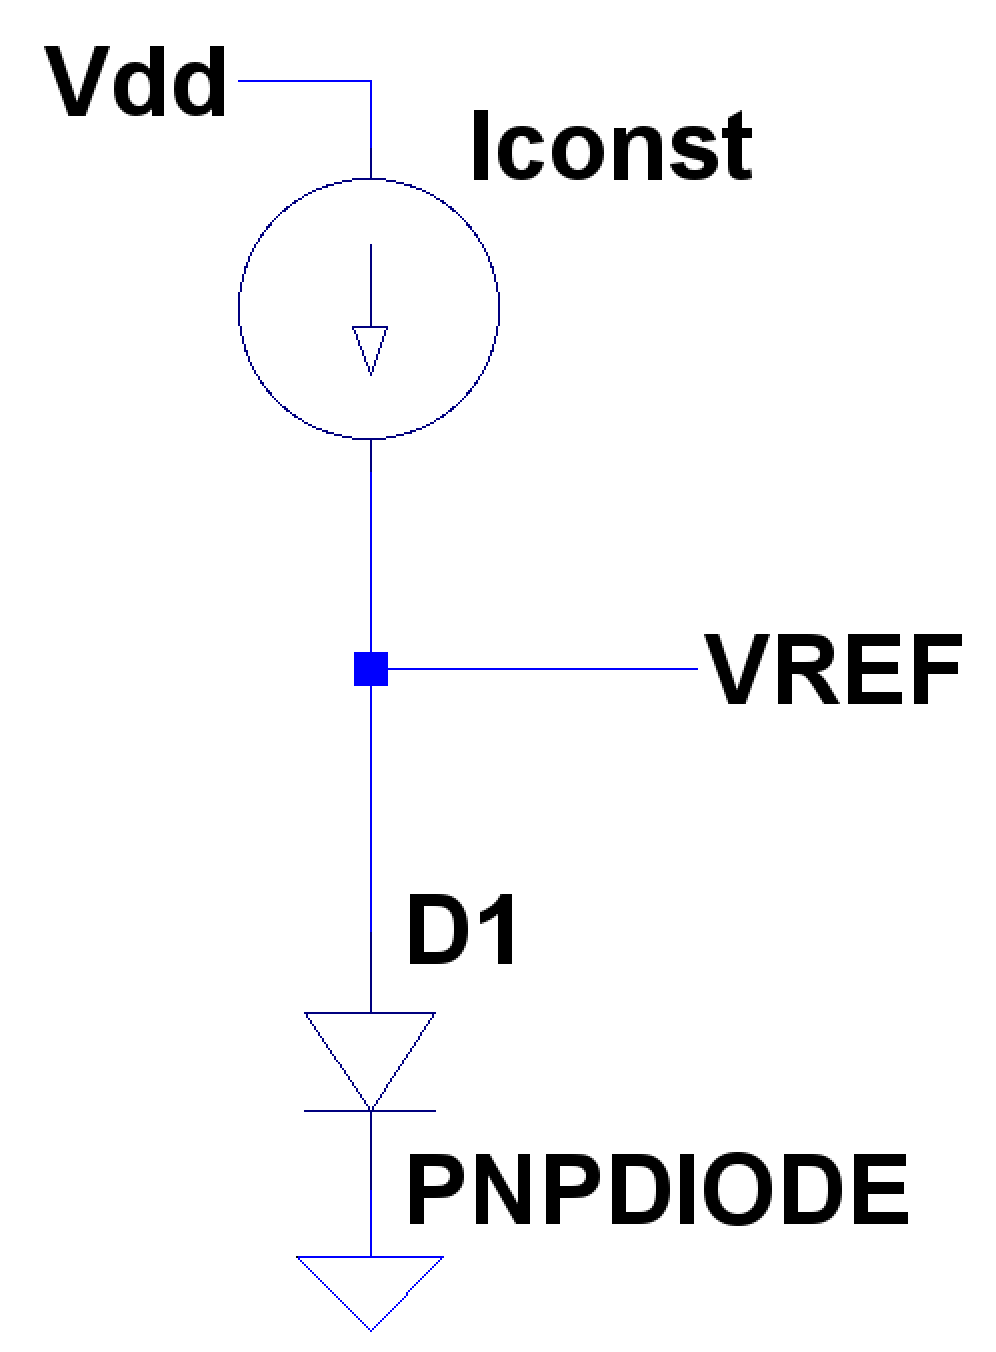
\includegraphics[scale=0.25]{images/cm-diode1.png}
  \caption[cm-diode1]{Current-Diode Circuit}
  \label{fig:cm-diode1}
\end{figure}
\begin{figure}[!htbp]
  \centering
  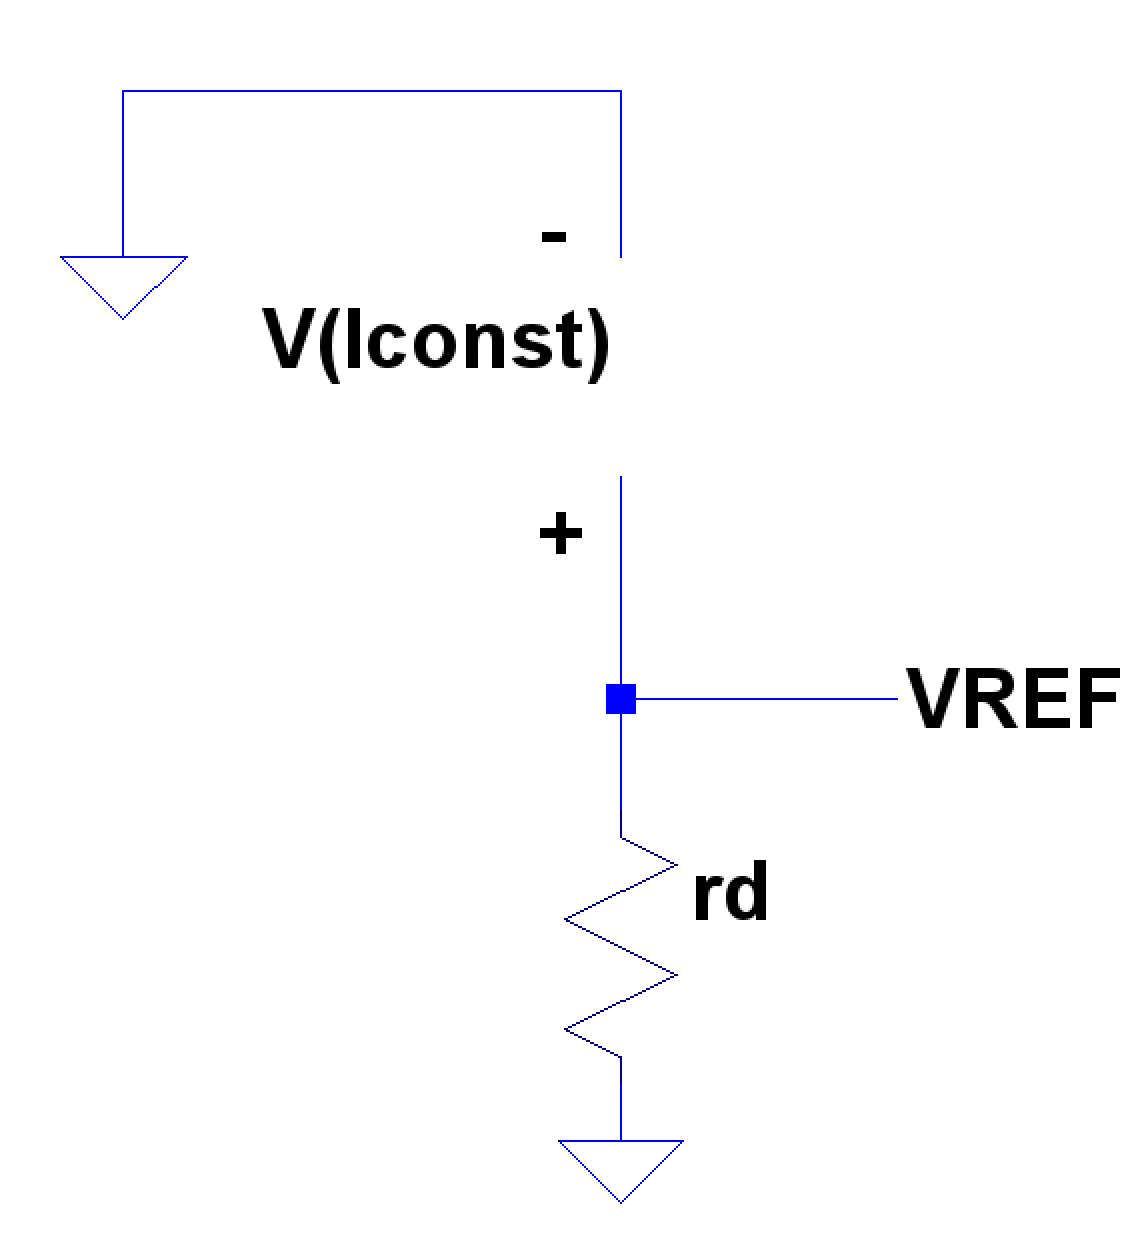
\includegraphics[scale=0.25]{images/cm-diode1-ss.png}
  \caption[cm-diode1-ss]{Current-Diode Circuit LFSSM}
  \label{fig:cm-diode1-ss}
\end{figure}

\subsection{Current-Diode Design Approach}
Table \ref{tab:cm-diode-designequations} gives the relevant design equations for the Current Diode Voltage Reference design.  Equation \ref{diode-v} gives the diode voltage for a given diode current at the given reference temperature ($20\;^{\circ}$C).  To achieve a low power design, we set $I_{const} = 1\mu$A; this sets the reference voltage to $V_{BE0}$ at $T_0$.  To find the temperature coefficient of $V_{ref}$ near our reference temperature, we take $\frac{\partial{V_{BE}}}{\partial{T}}$ with $J_C = J_{C0}$ due to the constant current source and divide by $V_{BE0}$.  This gives Equation \ref{vbe-tc} where $k$ is Boltzman's Constant, $m = 2.3$ and $V_{G0} = 1.206$ ($V$).

\begin{table}[!htbp]
  \caption[]{Current-Diode Design Equations}
  \label{tab:cm-diode-designequations}
  \centering
  \begin{tabular}{|m{1.5cm}|m{6.5cm}|}
    \hline
    \pbox{1.5cm}{\small SS Diode Impedance}&
    \begin{equation}
      r_{_d} = \frac{V_{_T}}{I_{_D}} = \frac{kT}{qI_{_D}}
    \end{equation}
    \\\hline
    \pbox{1.5cm}{{\small Input Resistance}} &
    \begin{equation}
      R_{_{in}} = \frac{V_{_T}}{I_{_T}} = \infty
    \end{equation}
    \\\hline
    \pbox{1.5cm}{{\small Output Resistance}} &
    \begin{equation}
      R_{_{out}} = \frac{V_{_T}}{I_{_T}} = r_{_d}
    \end{equation}
    \\\hline
    \pbox{1.5cm}{{\small Diode Current}} &
    \begin{equation}
      I_{_D} = I_se^{^{V_{_D}/V_{T}}} = I_se^{^{qV_{_D}/kT}}
	\label{diodecurrent}
    \end{equation}
    \\\hline
    \pbox{1.5cm}{{\small $V_{BE0}$}} &
    \begin{equation}
      V_{_{BE0}} = \frac{kT_{_0}ln(I_{_D}/I_s)}{q}
	\label{diode-v}
    \end{equation}
    \\\hline
    \pbox{1.5cm}{{\small $V_{BE}$}} &
    \begin{multline}
      V_{_{BE}} = V_{_{G0}}(1 - \frac{T}{T_{_0}}) + V_{_{BE0}}\frac{T}{T_{_0}}\\+ \frac{mkT}{q}ln(\frac{T_{_0}}{T}) + \frac{kT}{q}ln(\frac{J_{_c}}{J_{_{c0}}}) 
    \end{multline}
    \\\hline
    \pbox{1.5cm}{{\small $TC(V_{BE})$}} &
    \begin{multline}
      TC(V_{_{BE}}) = \frac{1}{V_{BE0}}[\frac{1}{T_0}(V_{BE0}-V_{G0})\\+
\frac{mk}{q}(\ln{\frac{T_o}{T}}-1)]
	\label{vbe-tc}
    \end{multline}
    \\\hline
  \end{tabular}
\end{table}

\subsection{Iteration 1}
	\subsubsection{Device Parameters}
\begin{table}[!htbp]
  \caption[]{Current Diode Voltage Reference, Iteration 1}
  \label{tab:cm-dp-1}
  \centering
  \begin{tabular}{|l|l|l|l|}
    \hline
    Parameter			& PNPDIODE	&Iconst	&R1	\\ \hline
    $R$ ($\Omega$)		&-			&-	&- 	\\ \hline
    $I_S$ (A)		&1e-18			&-	&-	\\ \hline
    $I$ ($\mu$A)	&-				&1	&-	\\
    \hline
  \end{tabular}
\end{table}

\subsection{Iteration 2}
	\subsubsection{Device Parameters}
\begin{table}[!htbp]
  \caption[]{Current Diode Voltage Reference, Iteration 2}
  \label{tab:cm-dp-2}
  \centering
  \begin{tabular}{|l|l|l|l|}
    \hline
    Parameter			& PNPDIODE	&Iconst	&R1	\\ \hline
    $R$ ($\Omega$)		&-			&-	&500k 	\\ \hline
    $I_S$ (A)		&1e-18			&-	&-	\\ \hline
    $I$ ($\mu$A)	&-				&1	&-	\\
    \hline
  \end{tabular}
\end{table}
%%END Current-Diode Voltage Divider

%%Begin Load Buffering
\section{Design 1-3 Load Buffering}
	\label{sec:Buff}

\begin{figure}[!htbp]
  	\centering
  	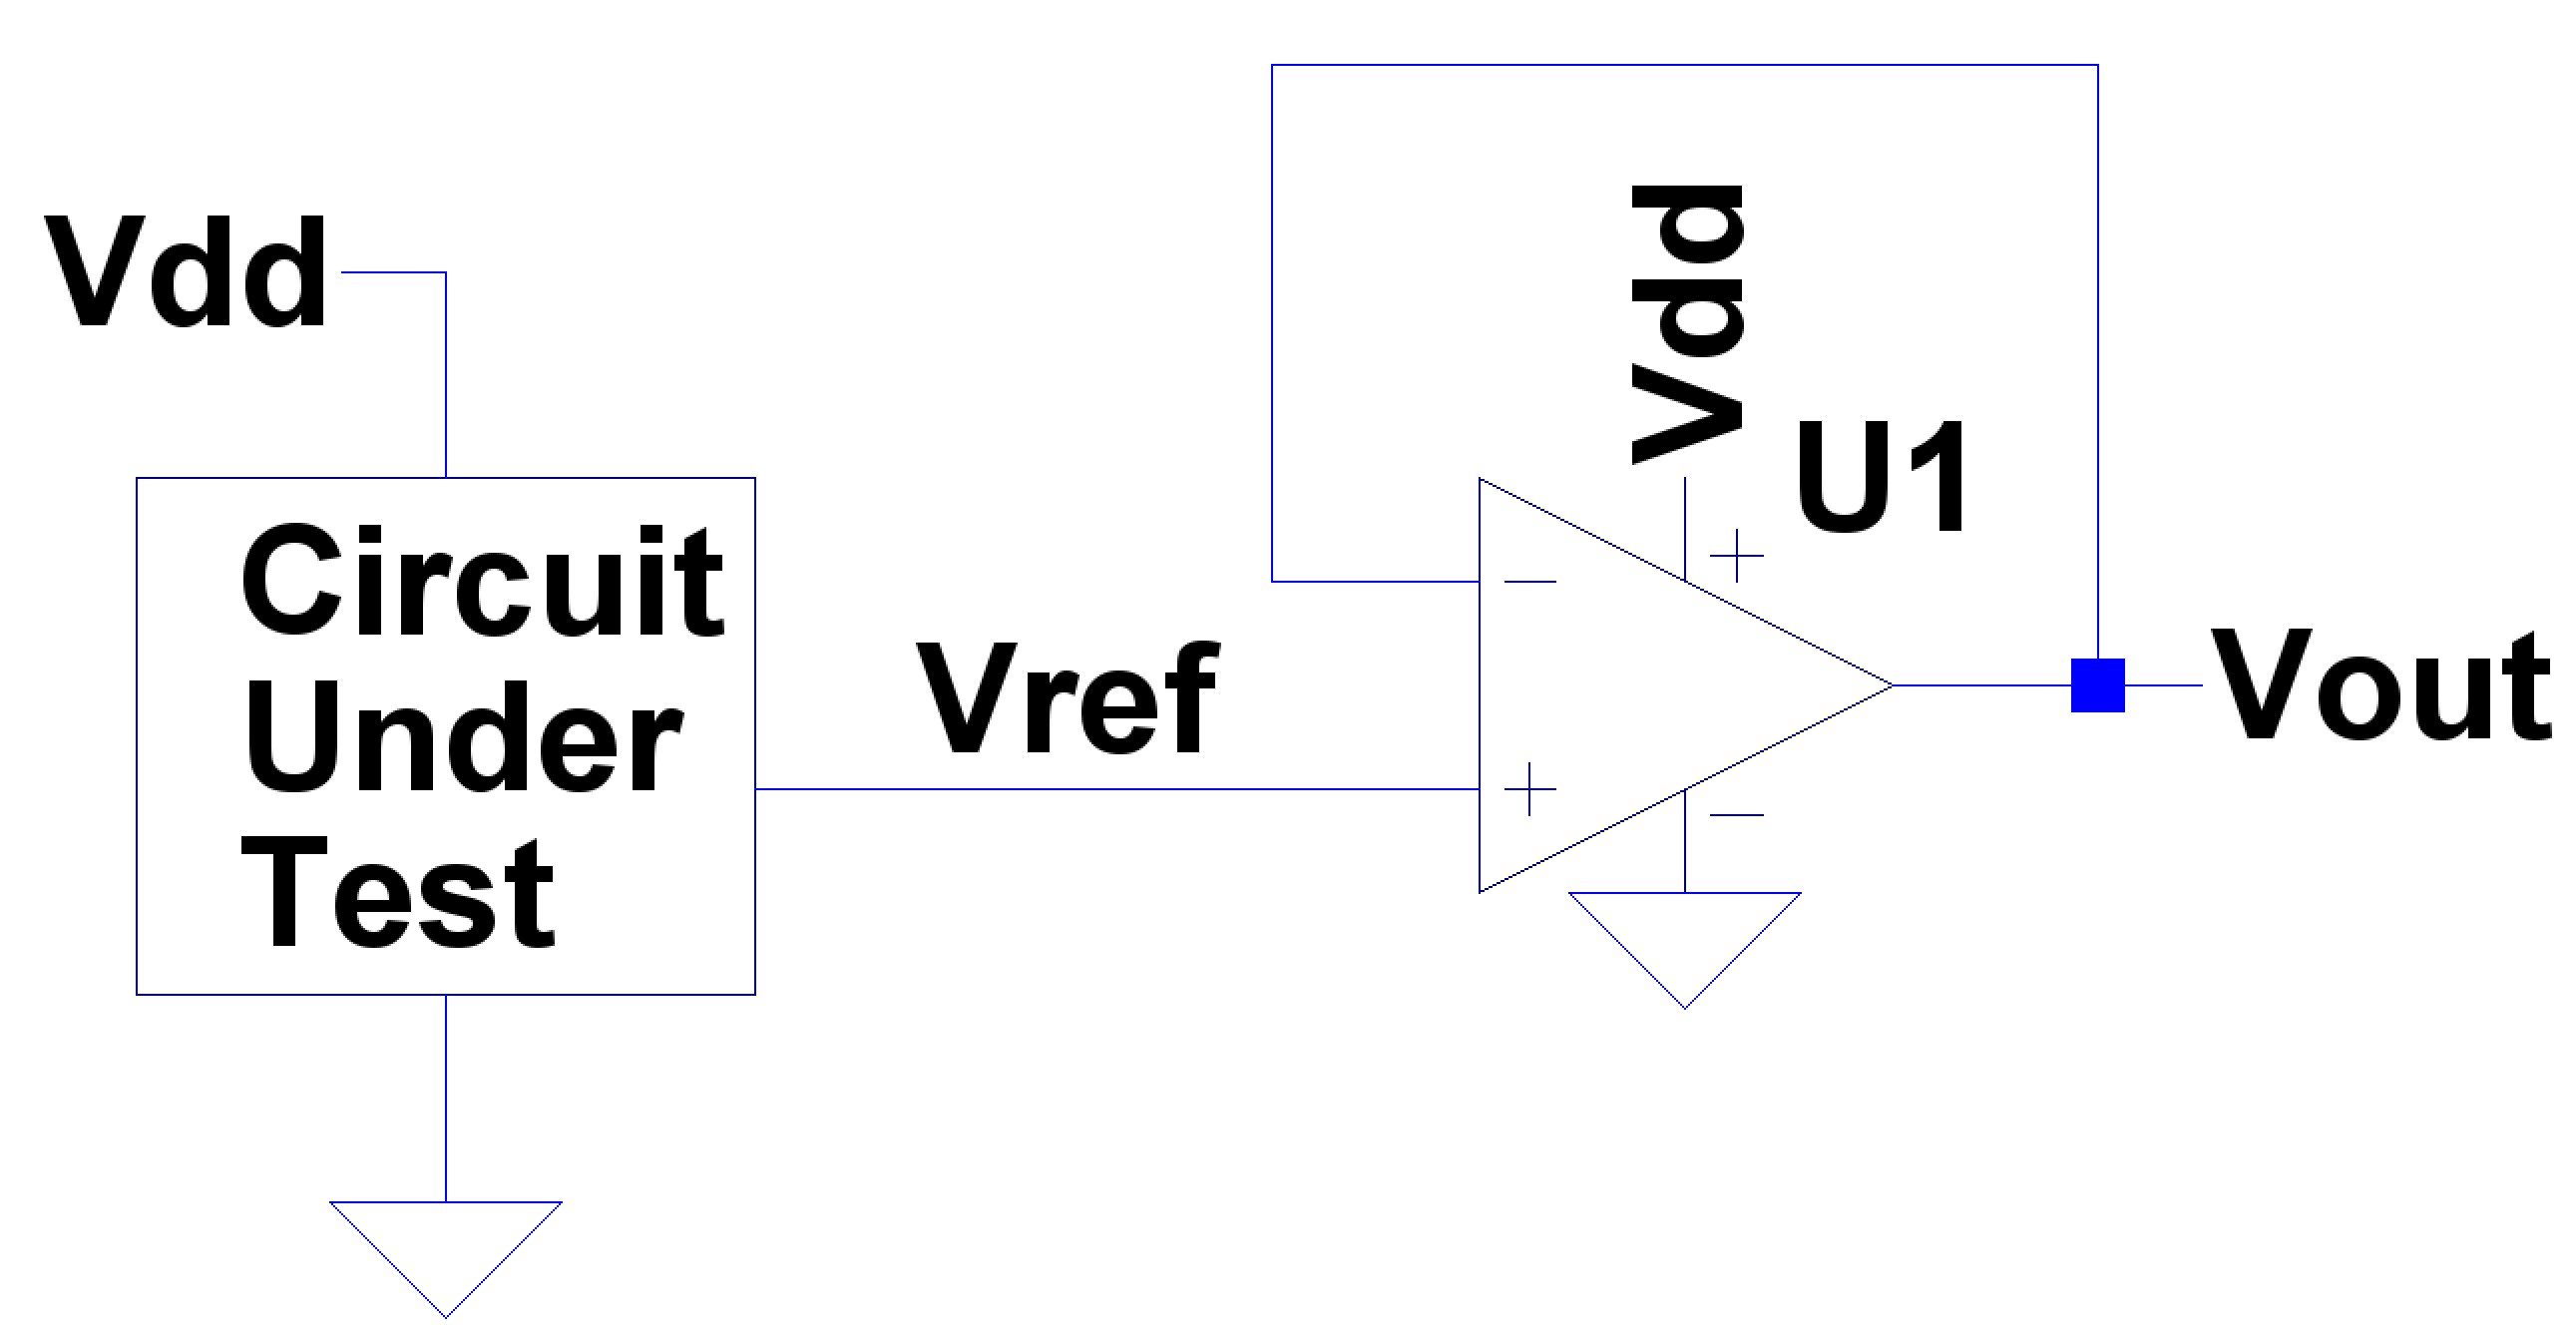
\includegraphics[scale=0.15]{images/loadbuff.png}
  	\caption[loadbuff]{Next Stage Load Buffering Circuit}
  	\label{fig:loadbuff}
	\end{figure}
%% END Load Buffering

%%Begin CMOS Bandgap Voltage Reference
\section{CMOS Bandgap Voltage Reference}
Figure \ref{fig:bgr-1} shows the generic CMOS Bandgap Voltage Reference. 

\begin{figure}[!htbp]
  	\centering
  	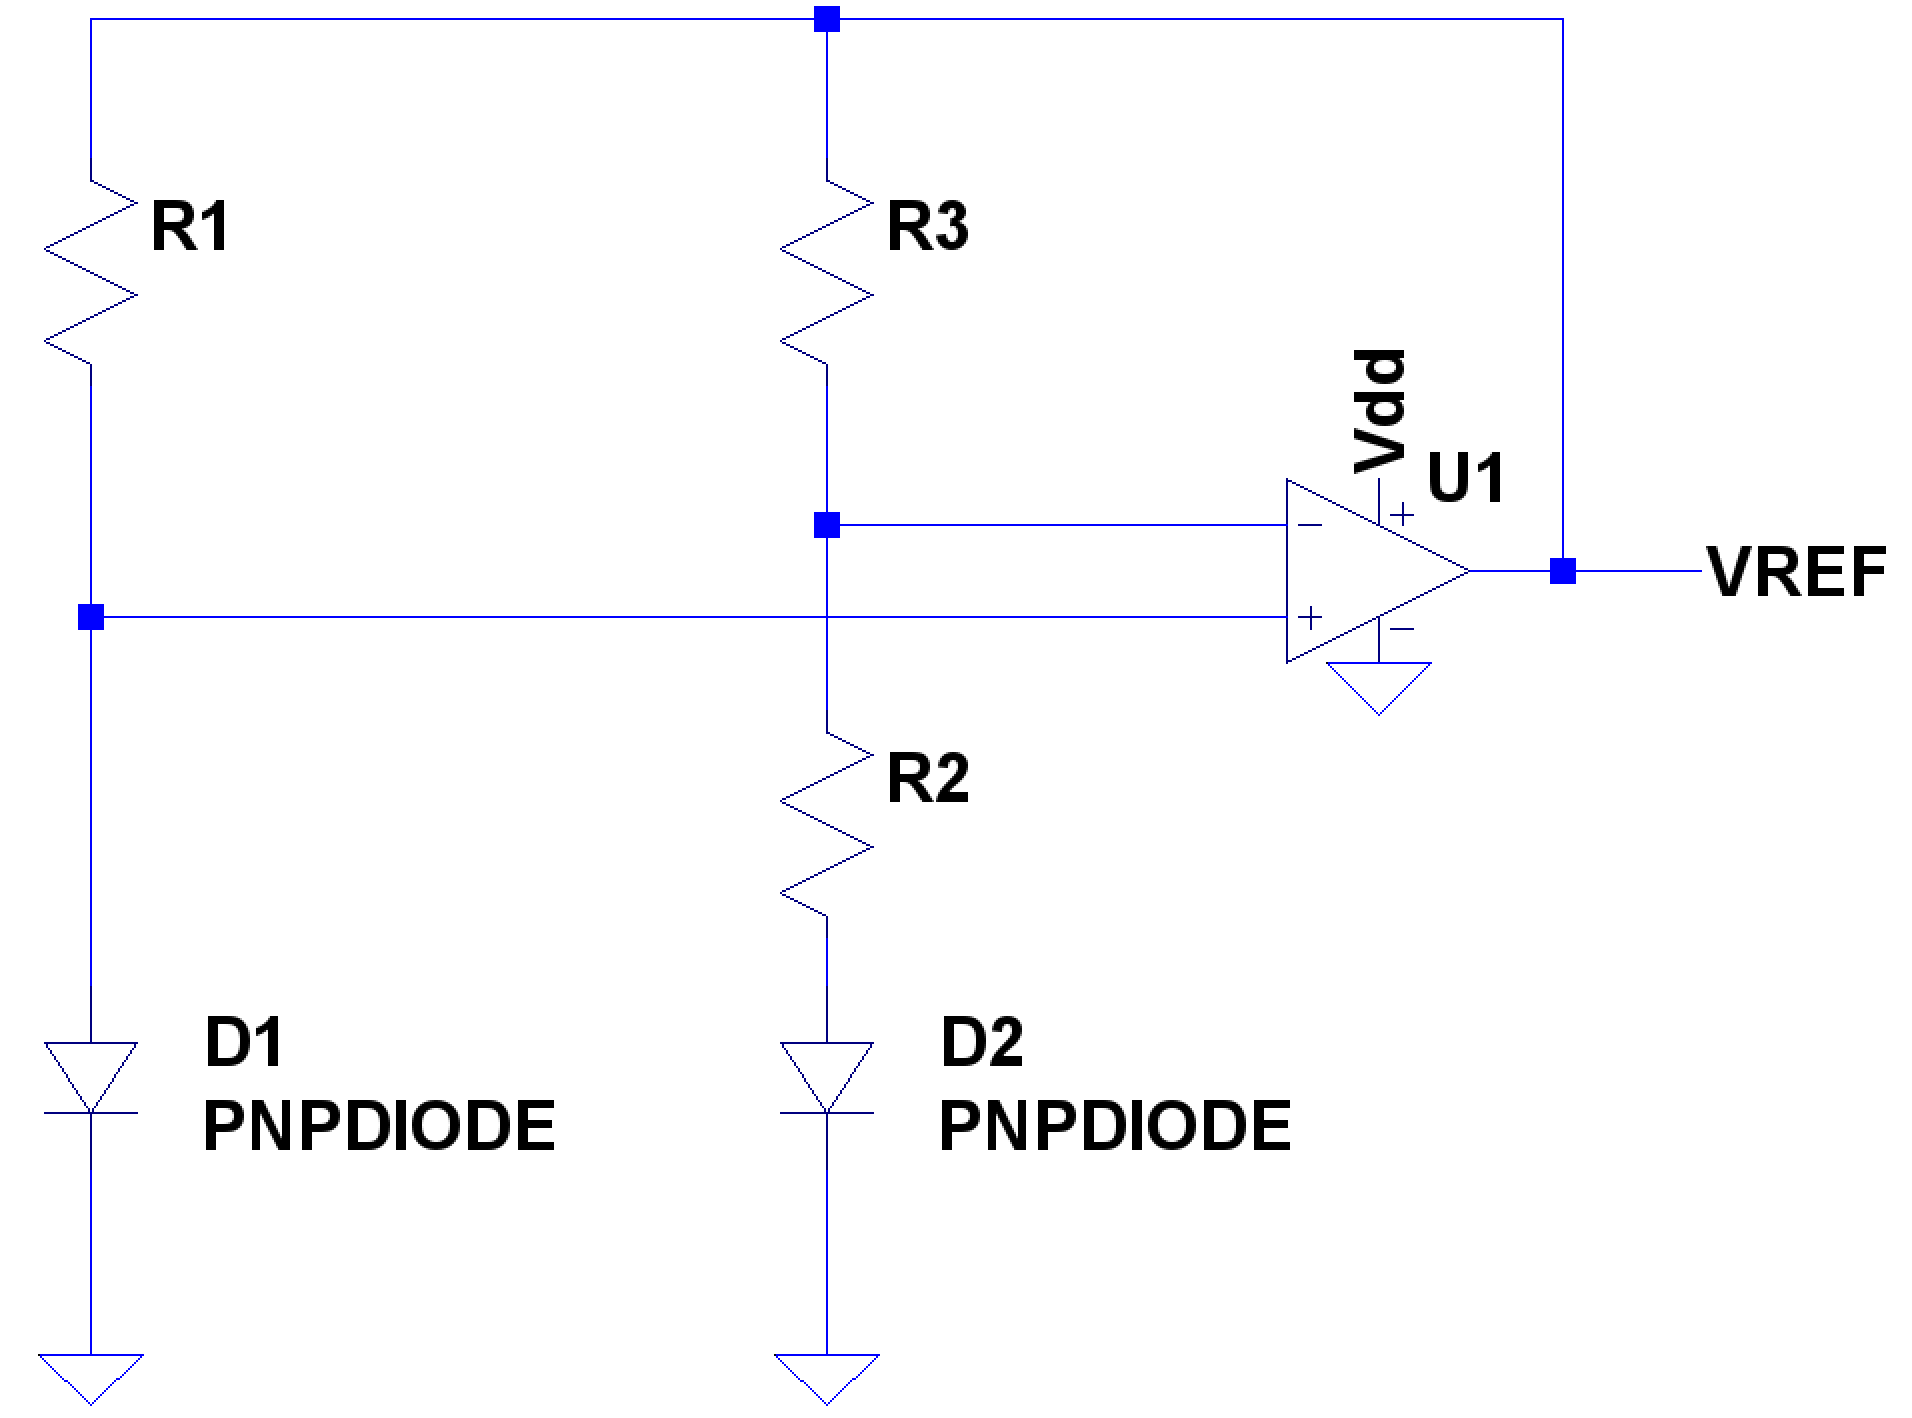
\includegraphics[scale=0.25]{images/bgr-1.png}
  	\caption[bgr-1]{CMOS Bandgap Voltage Reference Circuit}
  	\label{fig:bgr-1}
	\end{figure}

\subsection{Design Equations}

\subsection{Iteration 1}
	\subsubsection{Device Parameters}
\begin{table}[!htbp]
  \caption[]{Bandgap Reference Device Parameters, Iteration 1}
  \label{tab:bg-dp-1}
  \centering
  \begin{tabular}{|l|l|l|l|l|}
    \hline
    Parameter			& PNPDIODE	&R1 &R2	&R3 \\ \hline
    $R$ ($\Omega$)		&-			&1.69k	&2.13k	&16.9k\\ \hline
    $I_S$ (A)		&1e-18			&-	&-	&-\\
    \hline
  \end{tabular}
\end{table}

\subsection{Iteration 2}
	\subsubsection{Device Parameters}
\begin{table}[!htbp]
  \caption[]{Bandgap Reference Device Parameters, Iteration 2}
  \label{tab:bg-dp-2}
  \centering
  \begin{tabular}{|l|l|l|l|l|}
    \hline
    Parameter			& PNPDIODE	&R1 &R2	&R3 \\ \hline
    $R$ ($\Omega$)		&-		&	&	&\\ \hline
    $I_S$ (A)		&1e-18		&-	&-	&-\\
    \hline
  \end{tabular}
\end{table}
%%End CMOS Bandgap Voltage Reference

\onecolumn
%%Begin Sim Results/Comp
\section{Simulation and Results/Comparisons}
Figure \ref{fig:input-z-meas} in the Appendix shows the circuit for testing the input impedance of each circuit topology.  Figure \ref{fig:output-z-meas} in the Appendix shows the circuit for testing the output impedance of each circuit topology.  Figure \ref{fig:fr-meas} in the Appendix shows the circuit for testing the frequency response of each circuit topology.\\

\begin{table}[h]
  \caption[]{Resistor-MOSFET Voltage Divider Results}
  \label{tab:rm-res}
  \centering
    \begin{tabular}{|l|l|l|l|l|}
        \hline
        Parameter                & Hand-calc & Iteration 1 & Iteration 2 & Comments \\ \noalign{\hrule height 1.3pt}
        \# Passive Elements      & 1                 & 1           & 1           & ~        \\ \hline
        \# Active Elements       & 1                 & 1           & 1           & ~        \\ \hline
        $\sum$Width ($\mu$m)       & 3                 & 3           & 3           & ~        \\ \hline
        $\sum$Area ($\mu$m)$^2$    & 3                 & 3           & 3           & ~        \\ \noalign{\hrule height 1.3pt}
        $\sum P$ (m$W$)          & 0.500                 & 0.442           & 0.003          & ~        \\ \noalign{\hrule height 1.3pt}
        $V_{ref}$ ($V$)		      & 1.24                 & 1.314           & 0.466           & ~        \\ \hline
        TC(Vref) ($ppm$)      & 2,171                 & 616           & 3.5           & ~        \\ \hline
        $V_{DD}$ Sens.           & 0.267                 & 0.514           & 0.035           & ~        \\ \noalign{\hrule height 1.3pt}
        $Z_{out}$ ($\Omega$)     & 1.06k                 & 1.03k          & 30k           & ~        \\ \hline
        $Z_{in}$ ($\Omega$)      & 2k                & 4.12k           &854k           & ~        \\ \noalign{\hrule height 1.3pt}
        $V_{out,max}$ ($V$)      & 1.24                 & 1.37           & 0.468           & ~        \\ \hline
        $V_{out,min}$ ($V$)      & 1.24                 & 1.25           & 0.467           & ~        \\ \noalign{\hrule height 1.3pt}
        Gain ($dBV$)             & ~                 & ~           & ~           & ~        \\ \hline
        $BW$ (Hz)                & ~                 & ~           & ~           & ~        \\ \hline
        GBW ($dBV$Hz) & ~                 & ~           & ~           & ~        \\ \hline
    \end{tabular}
\end{table}
\newpage
\begin{table}[h]
  \caption[]{MOSFET-Only Voltage Divider Results}
    \label{tab:mo-res}
  \centering
    \begin{tabular}{|l|l|l|l|l|}
        \hline
        Parameter                & Hand-calc & Iteration 1 & Iteration 2 & Comments \\ \noalign{\hrule height 1.3pt}
        \# Passive Elements      & 0                 & 0           & 0           & ~        \\ \hline
        \# Active Elements       & 2                 & 2           & 2           & ~        \\ \hline
        $\sum$Width ($\mu$m)       & 10                 & 10           & ~           & ~        \\ \hline
        $\sum$Area ($\mu$m)$^2$    & 10                 & 10           & ~           & ~        \\ \noalign{\hrule height 1.3pt}
        $\sum P$ (m$W$)          & 0.1                 & 0.094           & ~           & ~        \\ \noalign{\hrule height 1.3pt}
        $V_{ref}$ ($V$)		      & 0.904                 & .894           & ~           & ~        \\ \hline
        TC(Vref) ($ppm$)      & 13.6                 & 120.4           & ~           & ~        \\ \hline
        $V_{DD}$ Sens.           & 1.0045                 & 0.5           & ~           & ~        \\ \noalign{\hrule height 1.3pt}
        $Z_{out}$ ($\Omega$)     & 101.25k                 & 2.3k           & ~           & ~        \\ \hline
        $Z_{in}$ ($\Omega$)      & -165                 & 10.4k           & ~           & ~        \\ \noalign{\hrule height 1.3pt}
        $V_{out,max}$ ($V$)      & 0.904                  & .903           & ~           & ~        \\ \hline
        $V_{out,min}$ ($V$)      & 0.904                  & .887           & ~           & ~        \\ \noalign{\hrule height 1.3pt}
        Gain ($dBV$)             & ~                 & ~           & ~           & ~        \\ \hline
        $BW$ (Hz)                & ~                 & ~           & ~           & ~        \\ \hline
        GBW ($dBV$Hz) & ~                 & ~           & ~           & ~        \\ \hline
    \end{tabular}
\end{table}
\newpage
\begin{table}[h]
  \caption[]{Current Diode Voltage Divider Results}
  \label{tab:cd-res}
  \centering
    \begin{tabular}{|l|l|l|l|l|}
        \hline
        Parameter                & Hand-calc & Iteration 1 & Iteration 2 & Comments \\ \noalign{\hrule height 1.3pt}
        \# Passive Elements      & 0                 & 0           & 1           & ~        \\ \hline
        \# Active Elements       & 1                 & 1           & 1           & ~        \\ \hline
        $\sum$Width ($\mu$m)       & -                 & -           & -           & -        \\ \hline
        $\sum$Area ($\mu$m)$^2$    & -                 & -           & -           & -        \\ \noalign{\hrule height 1.3pt}
        $\sum P$ (m$W$)          & 0.0018                 & 0.0018           & 0.0018           & $P$ is set by Id\\ \noalign{\hrule height 1.3pt}
        $V_{ref}$ ($V$)		      &0.698                & 0.725           & 1.216           & ~        \\ \hline
        TC(Vref) ($ppm$)      & -2,800                 &-2,160           & -137           & ~        \\ \hline
        $V_{DD}$ Sens.           & 0                 		& 0           & 0           & ~        \\ \noalign{\hrule height 1.3pt}
        $Z_{out}$ ($\Omega$)     & 25.3k                 & 25.9k           &525.9k           & ~        \\ \hline
        $Z_{in}$ ($\Omega$)      & $\infty$                 & $\infty$           & $\infty$           & ~        \\ \noalign{\hrule height 1.3pt}
        $V_{out,max}$ ($V$)      & 0.698                 & 0.833           & 1.23           & ~        \\ \hline
        $V_{out,min}$ ($V$)      & 0.698                 & 0.597           & 1.20          & ~        \\ \noalign{\hrule height 1.3pt}
        Gain ($dBV$)             & ~                 & ~           & ~           & ~        \\ \hline
        $BW$ (Hz)                & ~                 & ~           & ~           & ~        \\ \hline
        GBW ($dBV$Hz) & ~                 & ~           & ~           & ~        \\ \hline
    \end{tabular}
\end{table}
\begin{figure}[!htbp]
  	\centering
  	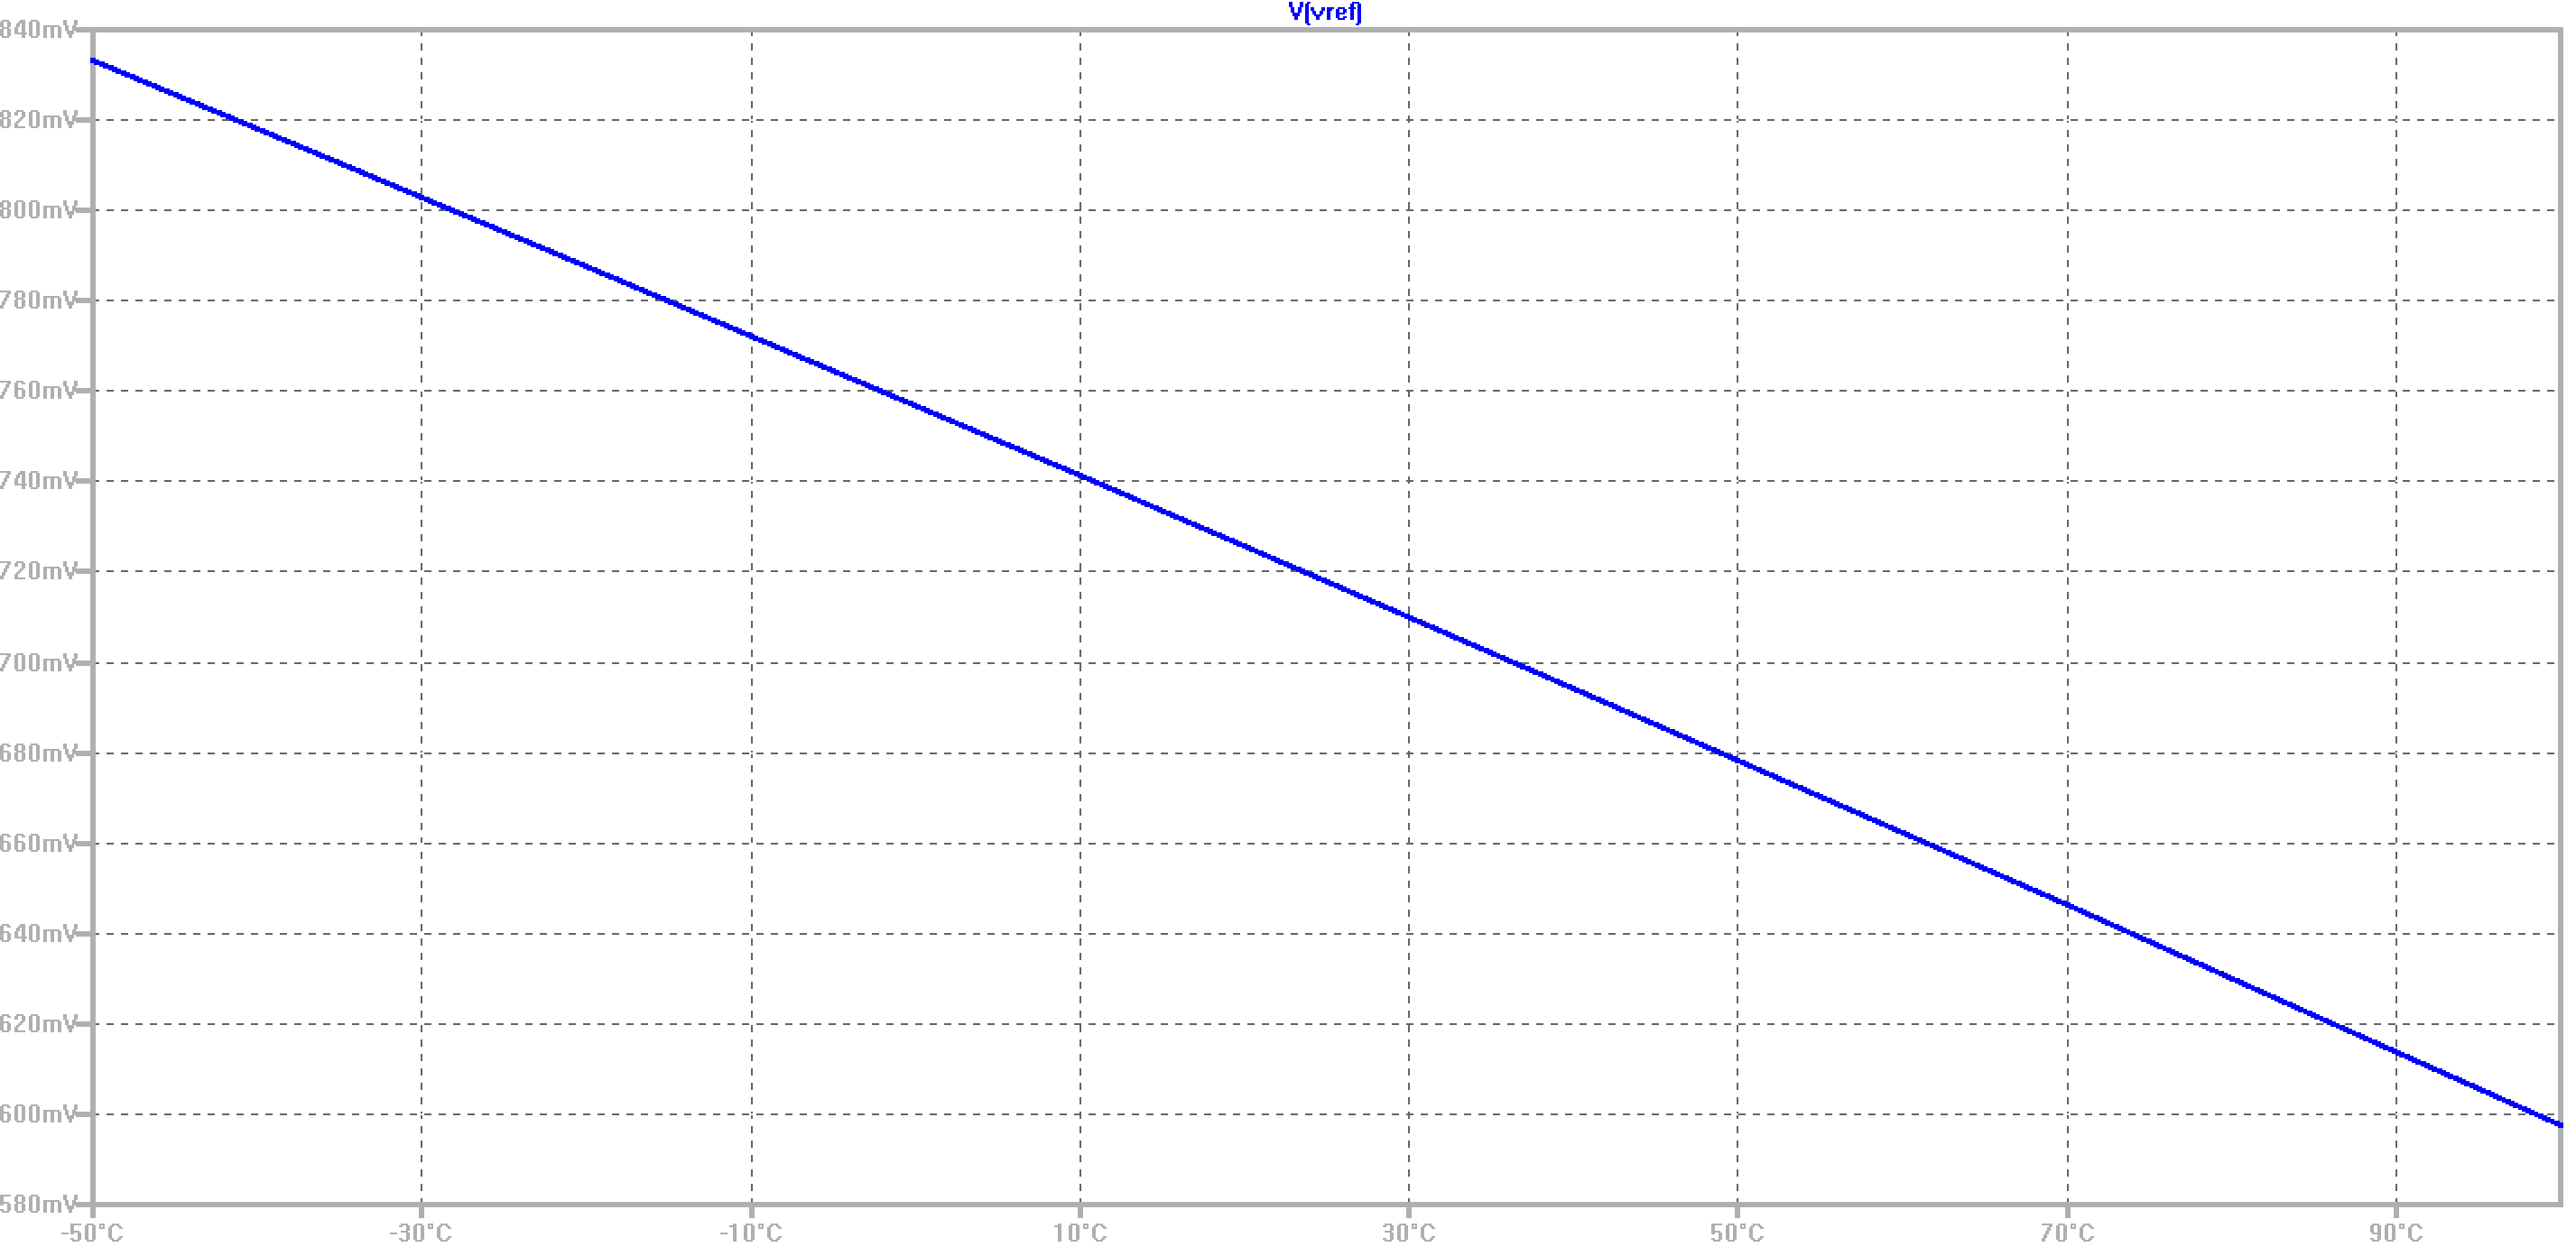
\includegraphics[scale=0.35]{images/cm-diode-vref-1.png}
  	\caption[cm-diode-vref-1]{Current Diode Voltage Reference VS Temperature, Iteration 1}
  	\label{fig:cm-diode-vref-1}
	\end{figure}

\begin{figure}[!htbp]
  	\centering
  	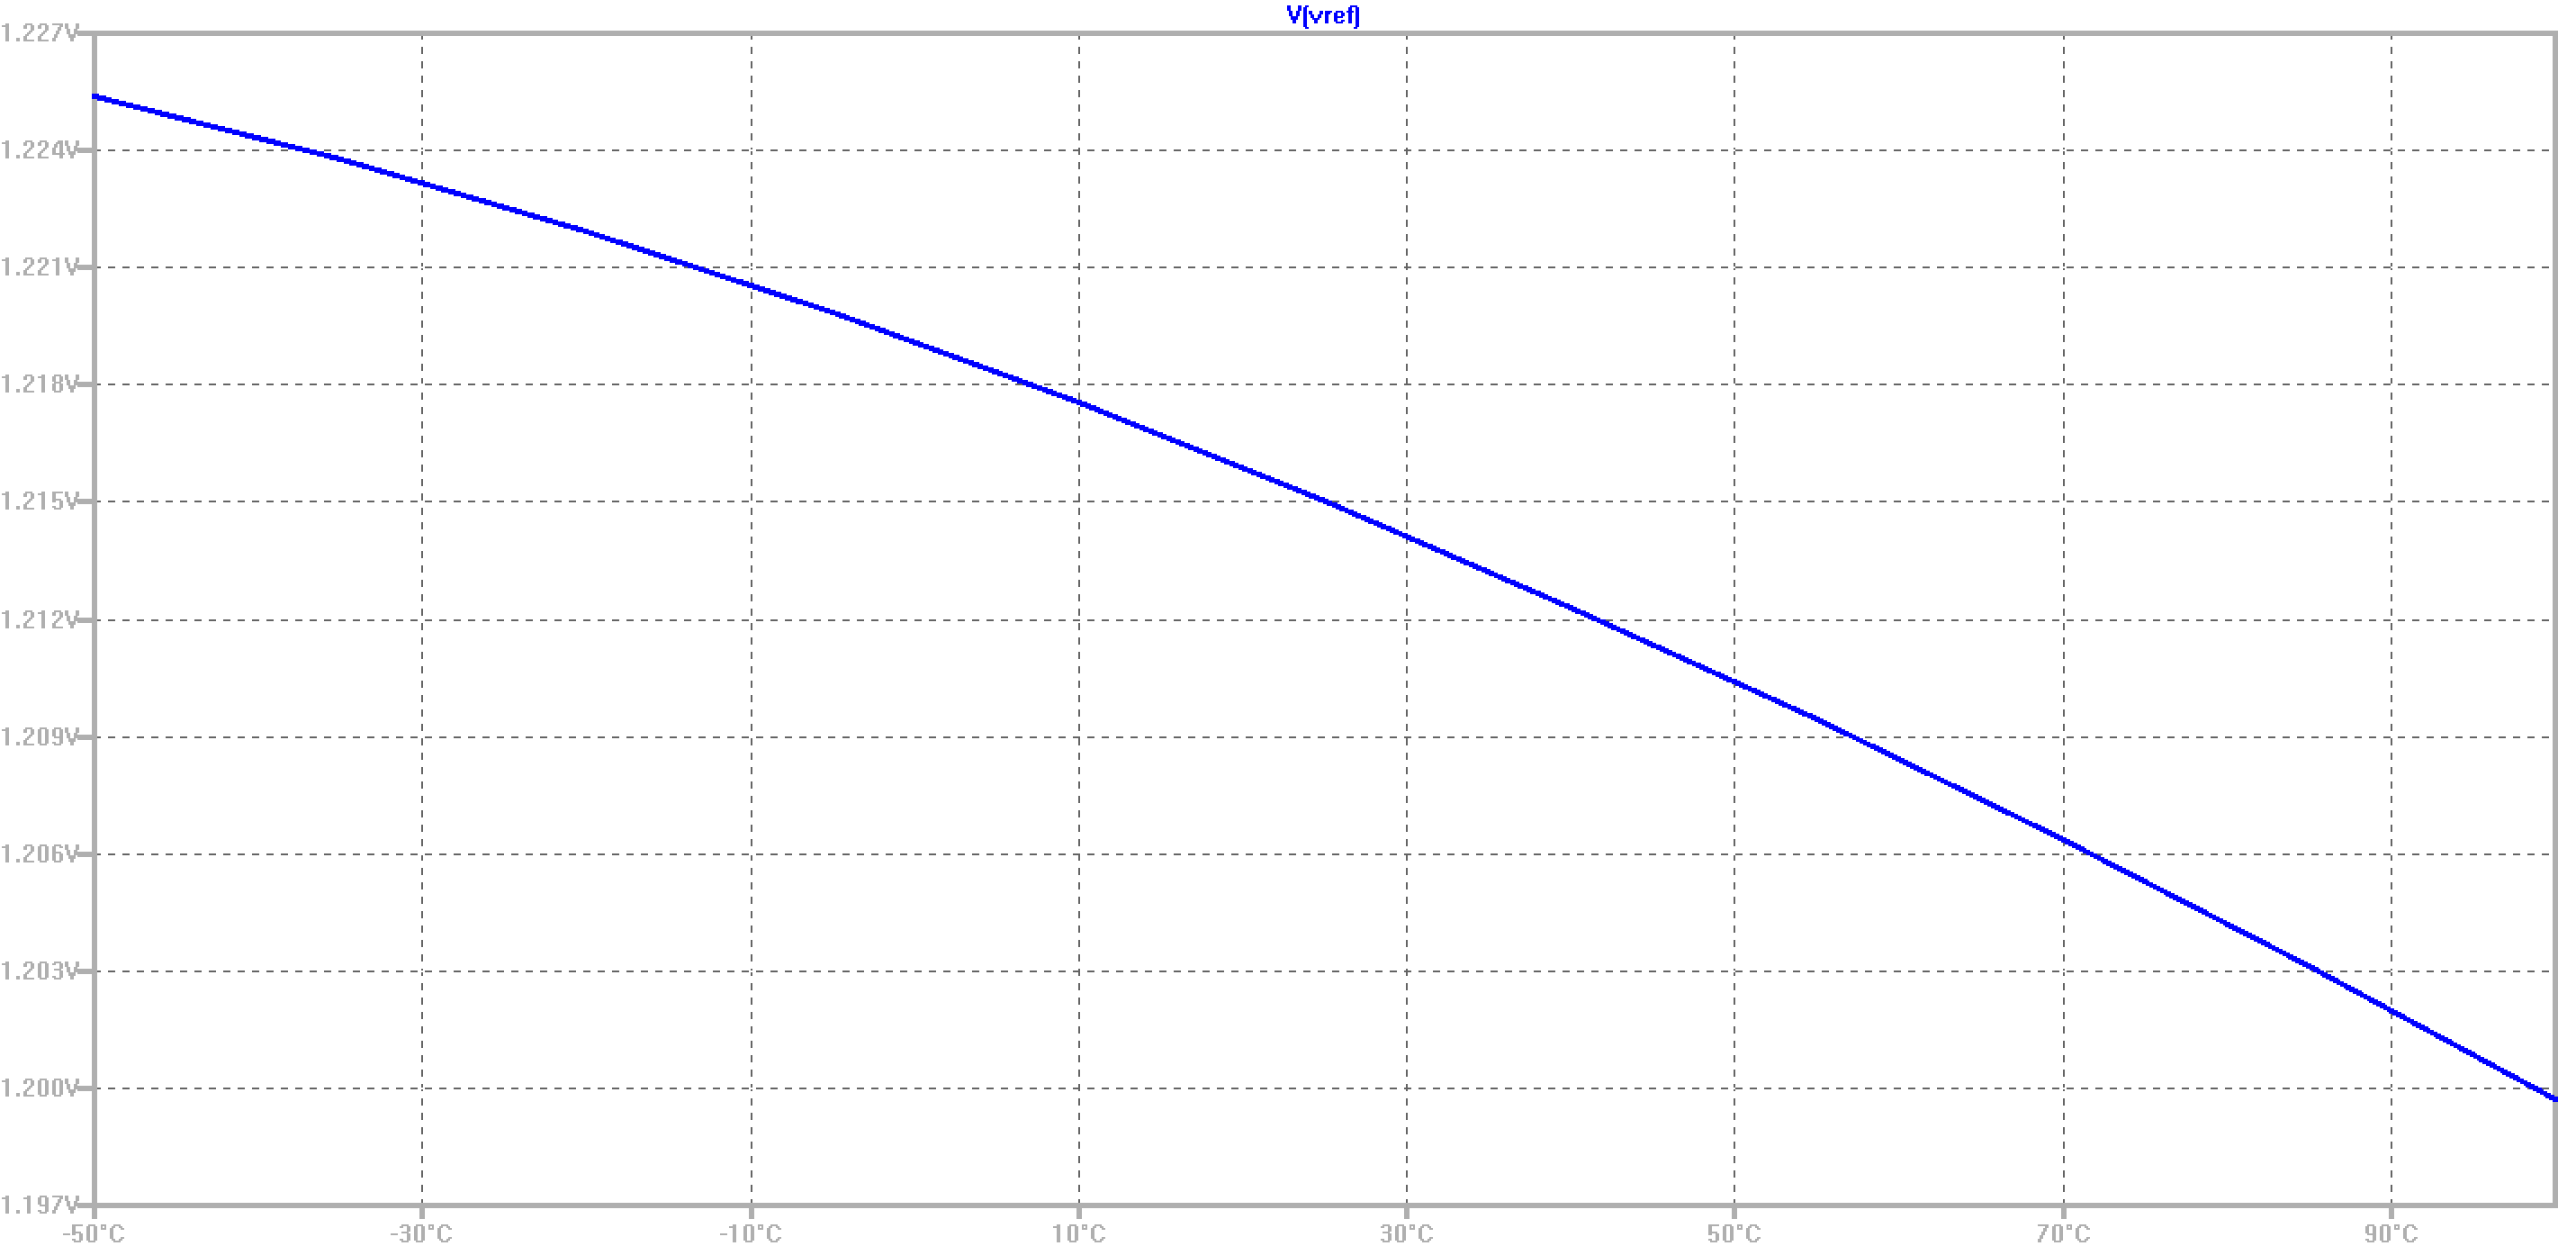
\includegraphics[scale=0.35]{images/cm-diode-vref-2.png}
  	\caption[cm-diode-vref-2]{Current Diode Voltage Reference VS Temperature, Iteration 2}
  	\label{fig:cm-diode-vref-2}
	\end{figure}
\begin{table}[h]
  \caption[]{CMOS Bandgap Voltage Reference Results}
  \label{tab:bgr-res}
  \centering
    \begin{tabular}{|l|l|l|l|l|}
        \hline
        Parameter                & Hand-calc & Iteration 1 & Iteration 2 & Comments \\ \noalign{\hrule height 1.3pt}
        \# Passive Elements      & 3                 & 3           & 3           & ~        \\ \hline
        \# Active Elements       & 3                 & 3           & 3           & ~        \\ \hline
        $\sum$Width ($\mu$m)       & -               & -           & -          & -        \\ \hline
        $\sum$Area ($\mu$m)$^2$    & -                 & -           & -           & -        \\ \noalign{\hrule height 1.3pt}
        $\sum P$ (m$W$)          & 1                 & 1.26           & ~           & ~        \\ \noalign{\hrule height 1.3pt}
        $V_{ref}$ ($V$)		      & 1.24                 & 1.33           & ~           & ~        \\ \hline
        TC(Vref) ($ppm$)      & 0                 & 396           & ~           & ~        \\ \hline
        $V_{DD}$ Sens.           & 0                 & 0.068           & ~           & ~        \\ \noalign{\hrule height 1.3pt}
        $Z_{out}$ ($\Omega$)     & 0                 & 72.7           & ~           & ~        \\ \hline
        $Z_{in}$ ($\Omega$)      & $\infty$                 &$\infty$            & ~           & ~        \\ \noalign{\hrule height 1.3pt}
        $V_{out,max}$ ($V$)      & 1.24                 & 1.37           & ~           & ~        \\ \hline
        $V_{out,min}$ ($V$)      & 1.24                & 1.29            & ~           & ~        \\ \noalign{\hrule height 1.3pt}
        Gain ($dBV$)             & -                 & ~           & ~           & ~        \\ \hline
        $BW$ (Hz)                & -                & ~           & ~           & ~        \\ \hline
        GBW ($dBV$Hz) 	& -                 & ~           & ~           & ~        \\ \hline
    \end{tabular}
\end{table}
%%END Sim Results/Comp

\twocolumn
%%Begin Conclusion
\section{Conclusion}
The conclusion goes here.
%%END Conclusion

\appendix
\label{app:A}
\begin{figure}[!htbp]
  	\centering
  	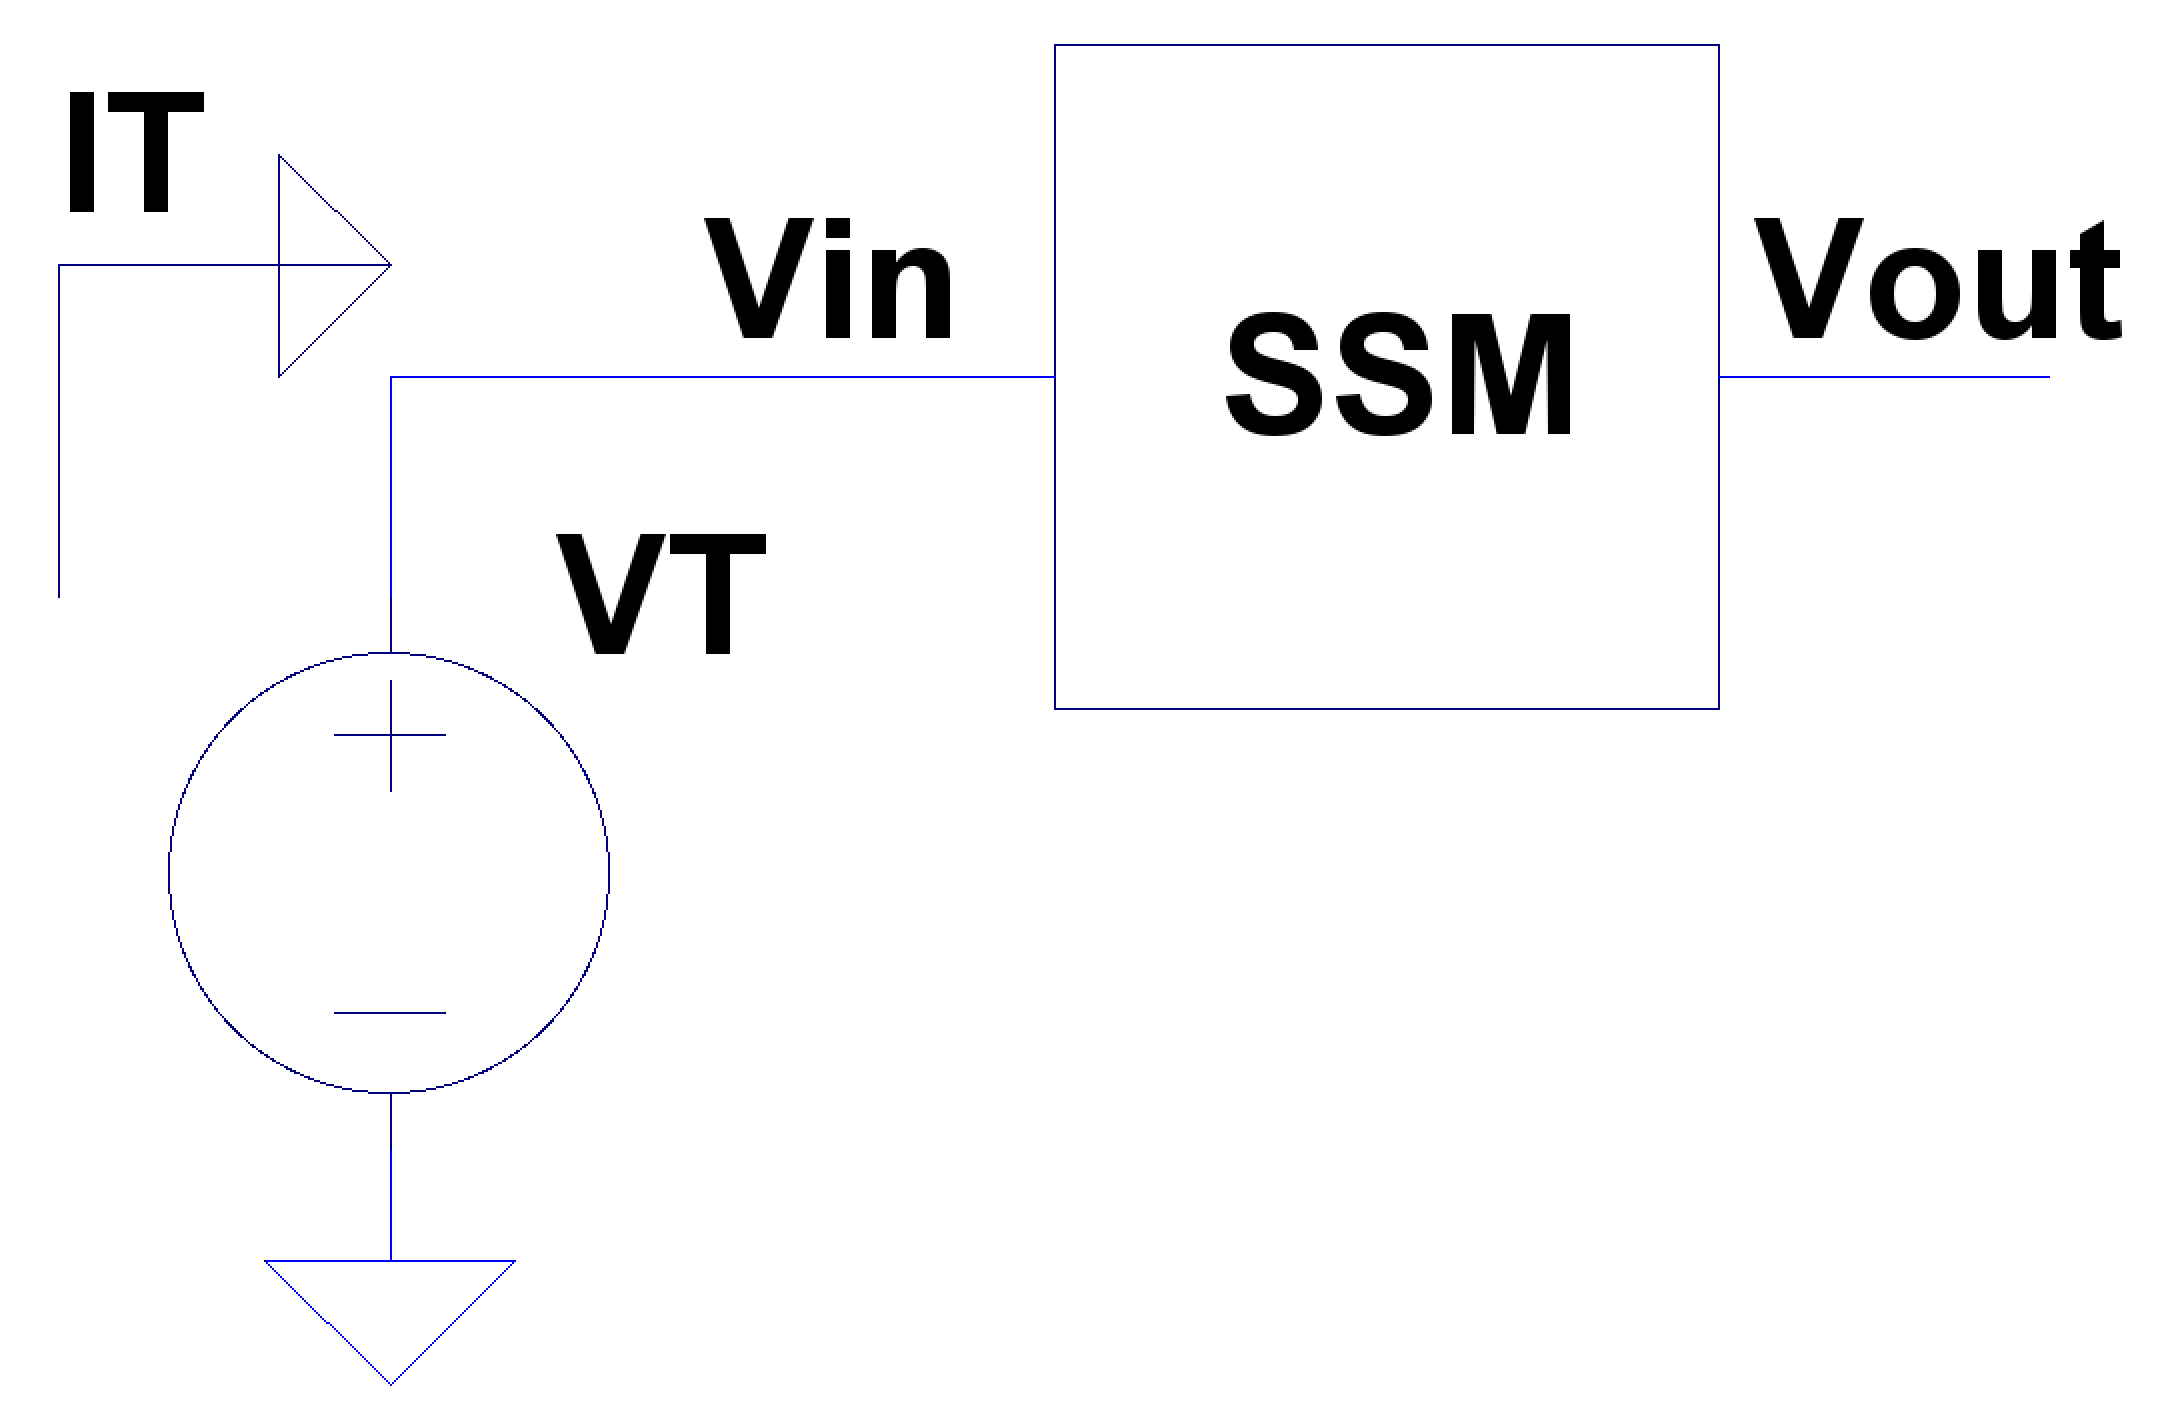
\includegraphics[scale=0.15]{images/input-z-meas.png}
  	\caption[input-z-meas]{Input Impedance Measurement Circuit}
  	\label{fig:input-z-meas}
	\end{figure}

\begin{figure}[!htbp]
  	\centering
  	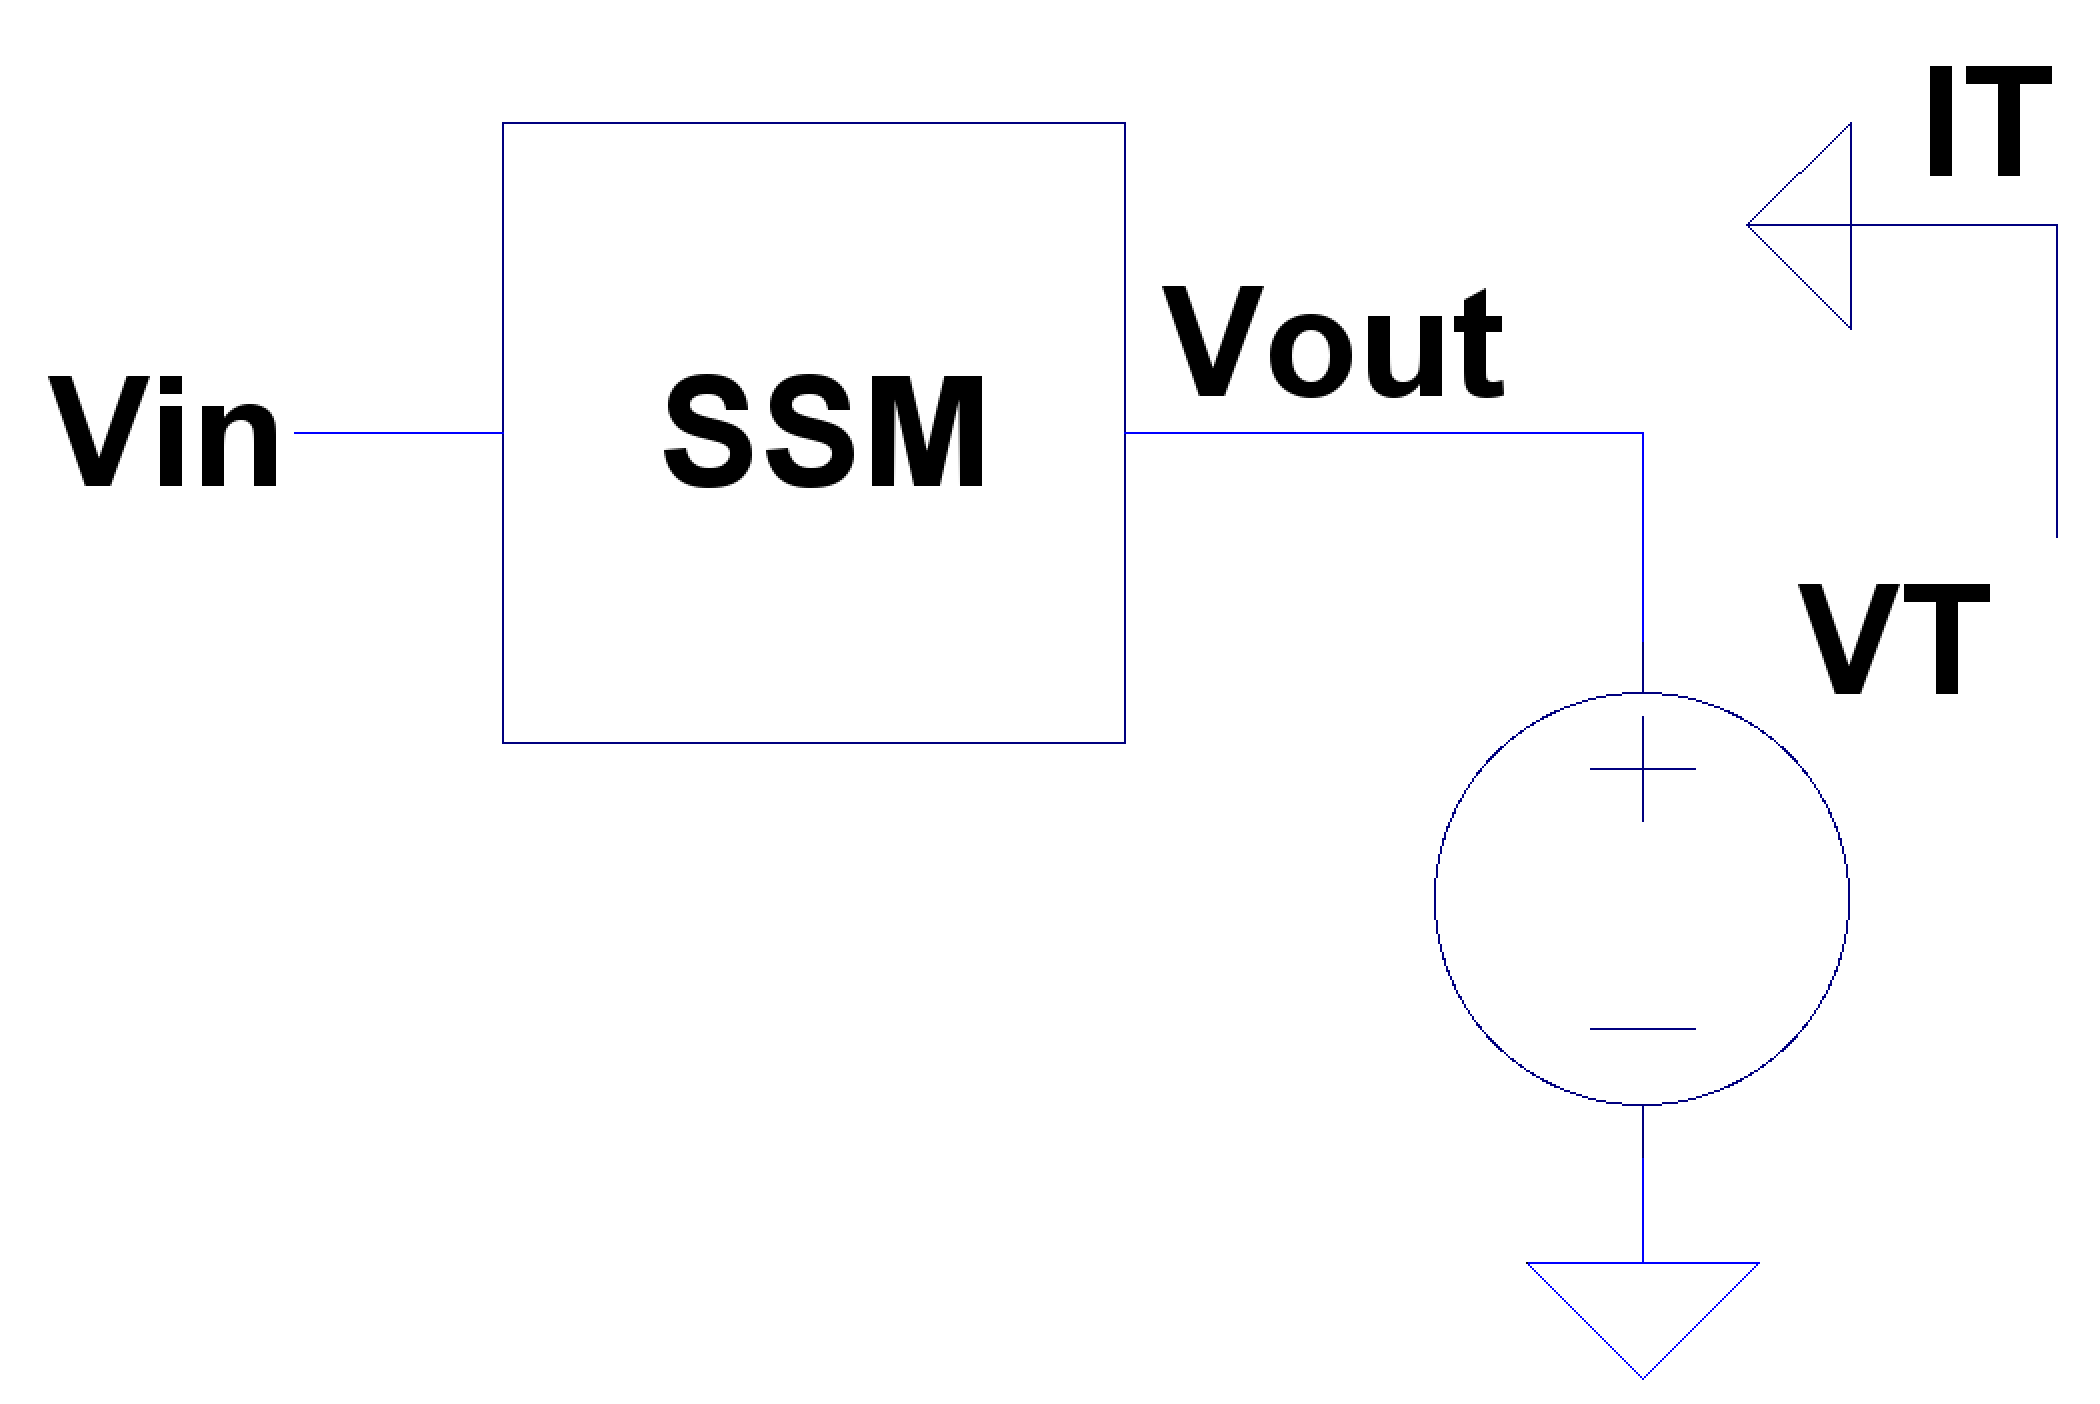
\includegraphics[scale=0.15]{images/output-z-meas.png}
  	\caption[output-z-meas]{Output Impedance Measurement Circuit}
  	\label{fig:output-z-meas}
	\end{figure}

\begin{figure}[!htbp]
  	\centering
  	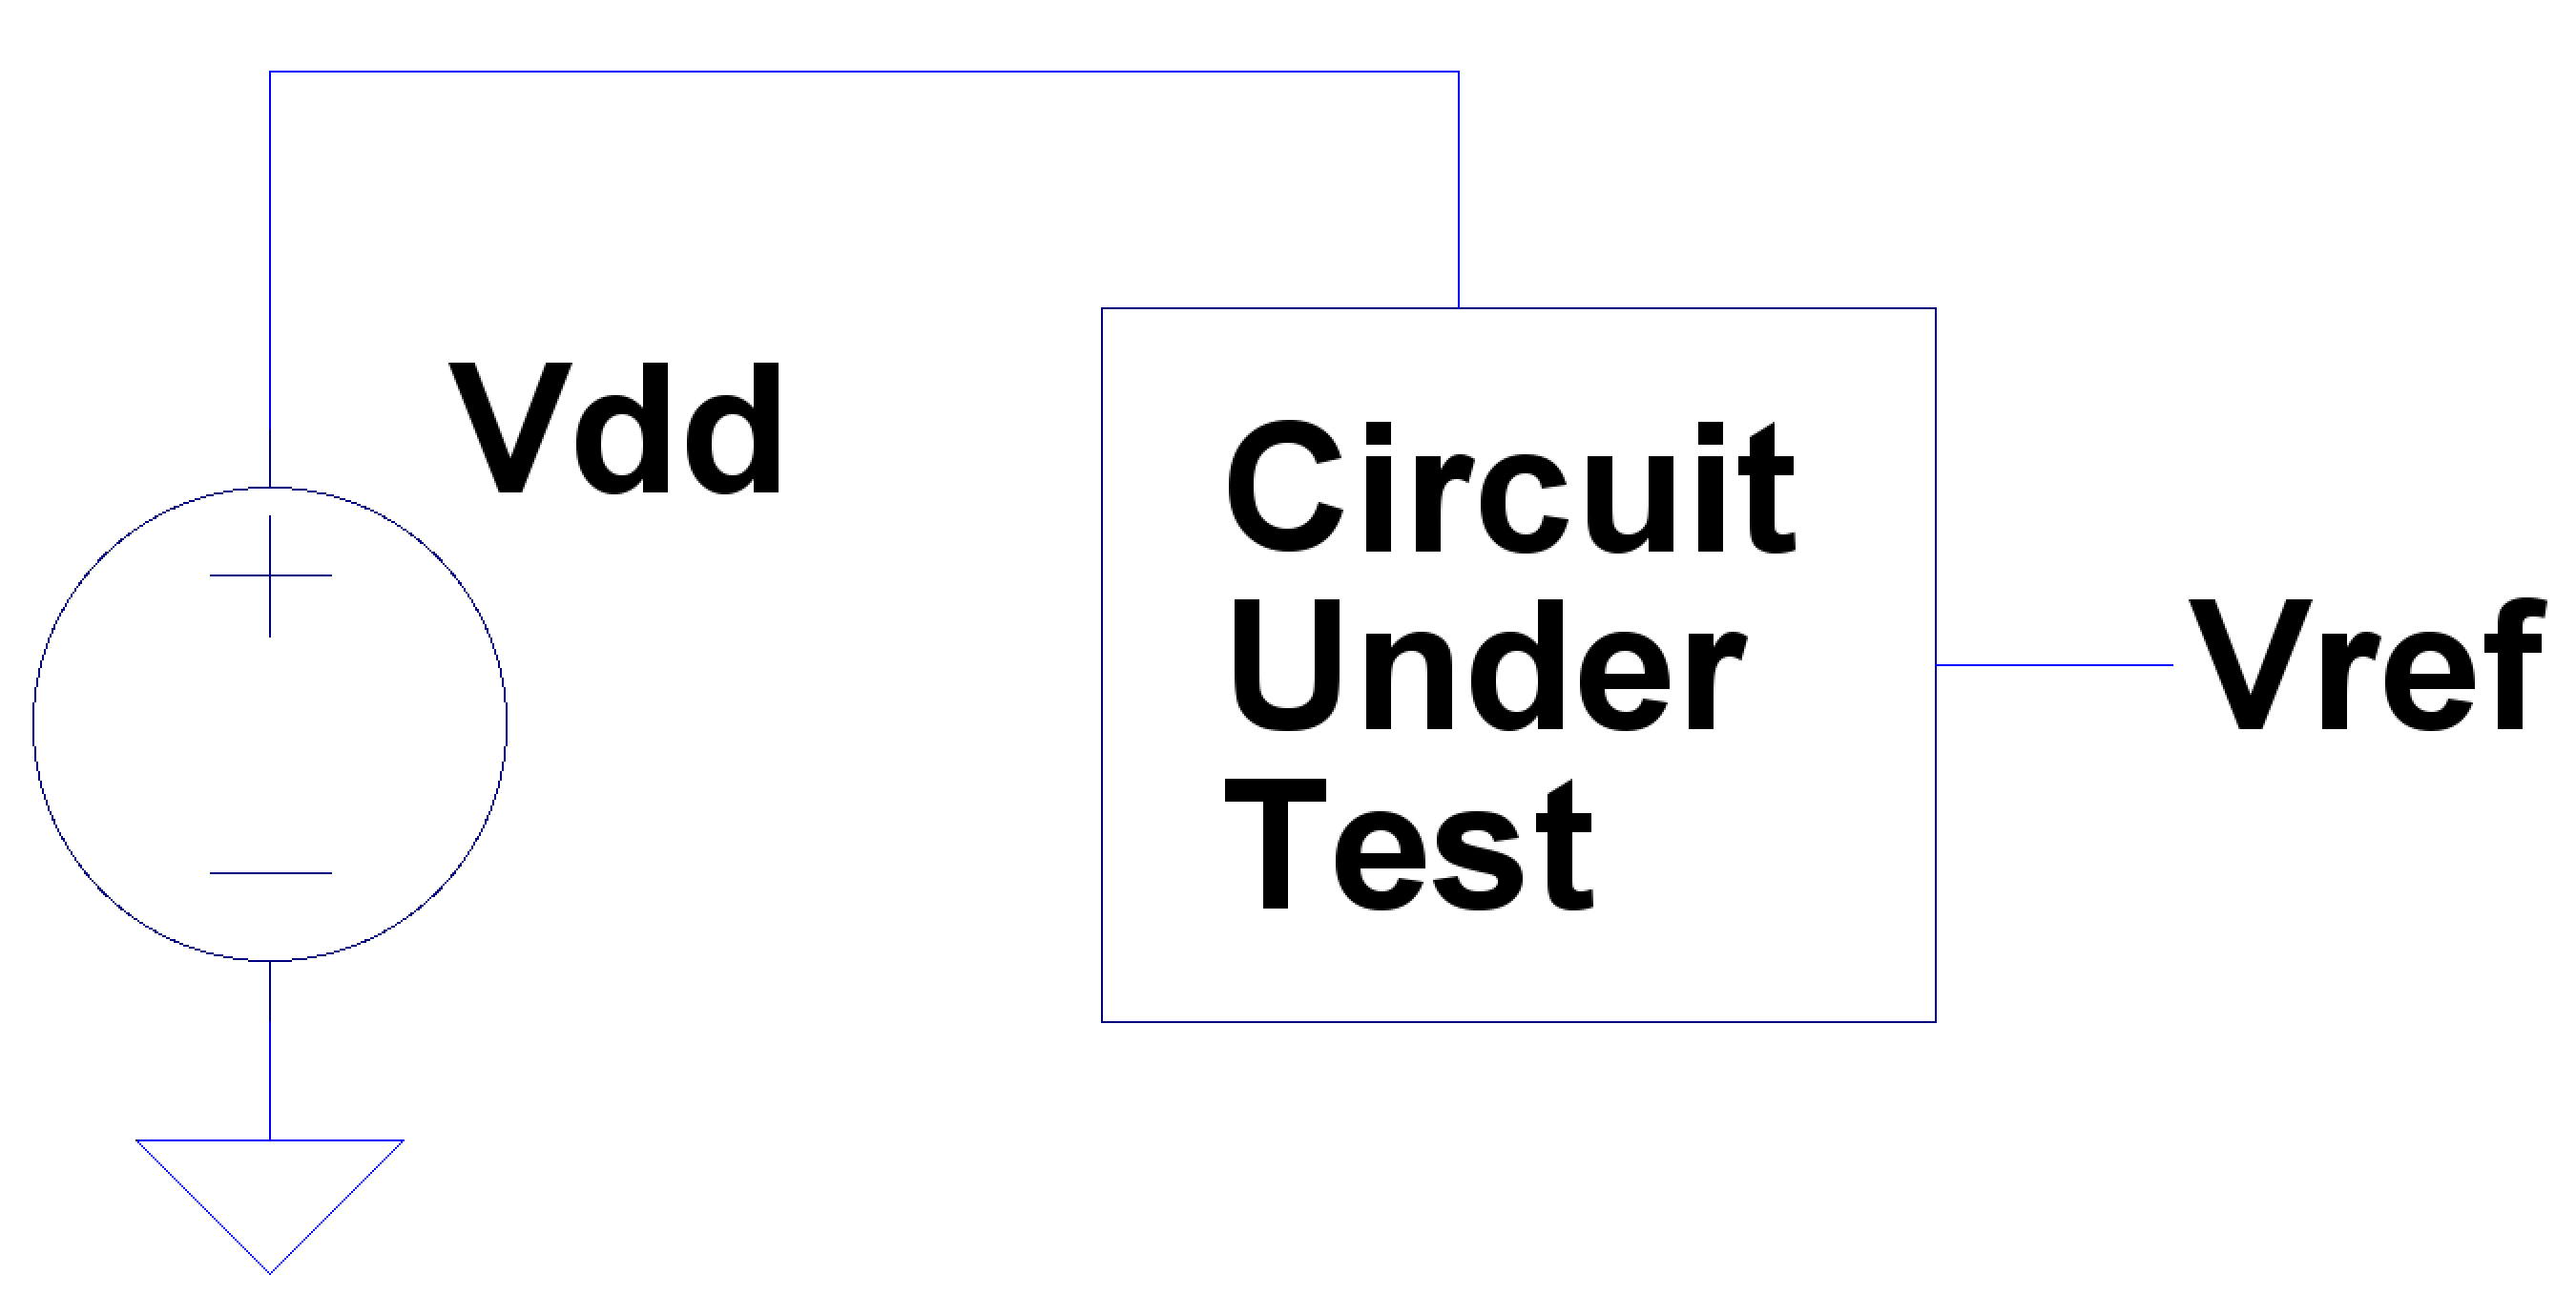
\includegraphics[scale=0.15]{images/sensitivity-meas.png}
  	\caption[sensitivity-meas]{$V_{DD}$ Sensitivity Measurement Circuit}
  	\label{fig:sensitiviy-meas}
	\end{figure}

\begin{figure}[!htbp]
  	\centering
  	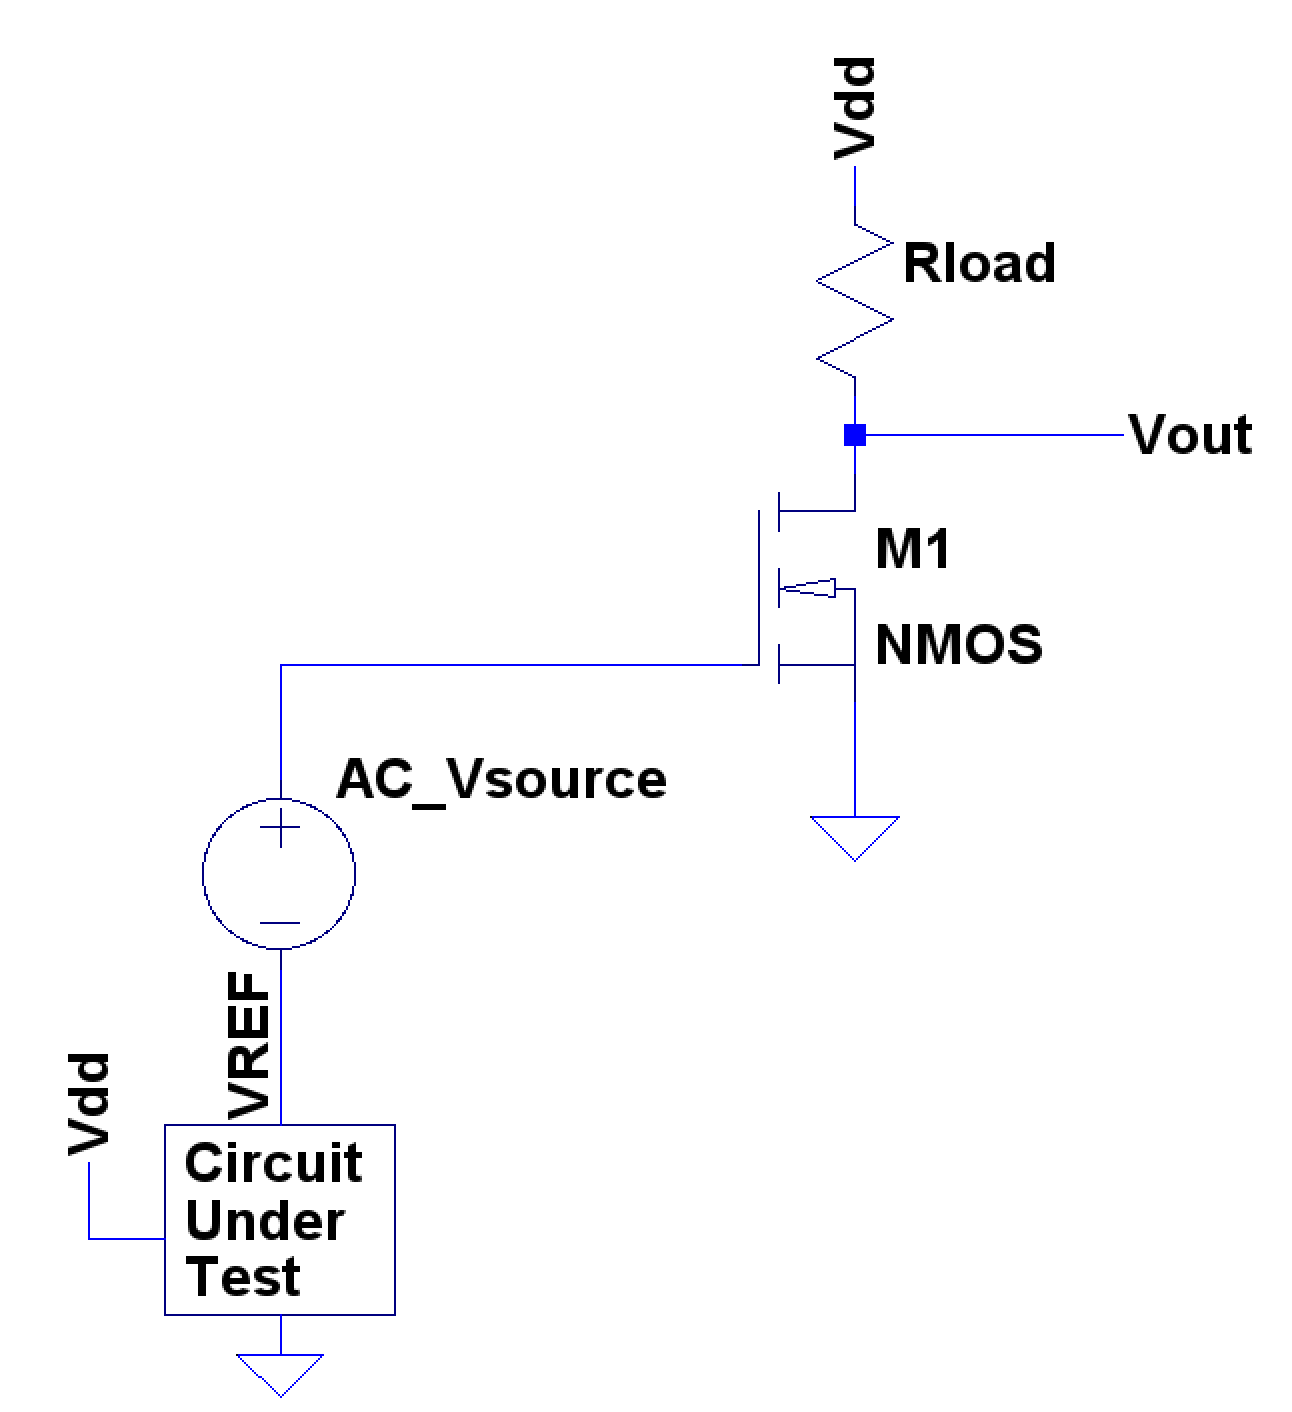
\includegraphics[scale=0.25]{images/fr-meas.png}
  	\caption[fr-meas]{Frequency Response Measurement Circuit}
  	\label{fig:fr-meas}
	\end{figure}


% conference papers do not normally have an appendix

%The authors would like to thank...
% trigger a \newpage just before the given reference
% number - used to balance the columns on the last page
% adjust value as needed - may need to be readjusted if
% the document is modified later
%\IEEEtriggeratref{8}
% The "triggered" command can be changed if desired:
%\IEEEtriggercmd{\enlargethispage{-5in}}

% references section

% can use a bibliography generated by BibTeX as a .bbl file
% BibTeX documentation can be easily obtained at:
% http://www.ctan.org/tex-archive/biblio/bibtex/contrib/doc/
% The IEEEtran BibTeX style support page is at:
% http://www.michaelshell.org/tex/ieeetran/bibtex/
%\bibliographystyle{IEEEtran}
% argument is your BibTeX string definitions and bibliography database(s)
%\bibliography{IEEEabrv,../bib/paper}
%
% <OR> manually copy in the resultant .bbl file
% set second argument of \begin to the number of references
% (used to reserve space for the reference number labels box)
\newpage
\begin{thebibliography}{1}
\bibitem{IEEEhowto:cmos_baker}
R. Jacob Baker, "CMOS: Circuit Design, Layout, and Simulation", 3rd edition, Wiley-IEEE Press, 2010

\bibitem{IEEEhowto:analog_carusone}
T. Chan Carusone, D. Johns, and K. Martin, "Analog Integrated Circuit Design," 2nd edition, J. Wiley \& Sons, 2011.
\end{thebibliography}
\end{document}
